\documentclass[conference, onecolumn]{IEEEtran}
% \IEEEoverridecommandlockouts
% The preceding line is only needed to identify funding in the first footnote. If that is unneeded, please comment it out.
\usepackage[T1]{fontenc}
\usepackage[margin=1.5in,marginpar=1.25in]{geometry}
\usepackage{lmodern}
\usepackage{cite}
\usepackage{IMTtikz}
\usepackage[hidelinks,colorlinks=true,urlcolor=blue,linkcolor=black,citecolor=blue]{hyperref}

\usepackage{polyglossia}

\setdefaultlanguage{english}
\SetLanguageKeys{english}{indentfirst=false}

\usepackage[english]{cleveref}
\crefformat{footnote}{#2\footnotemark[#1]#3}

\usepackage{algorithmic}
\usepackage{multicol,multirow,makecell}
\usepackage{caption}
% \usepackage{listings}
\usepackage{graphicx}
\usepackage{float}
\usepackage{textcomp}
\usepackage{xcolor}
\usepackage{booktabs}
\usepackage{setspace}
\usepackage[obeyFinal]{todonotes}

\definecolor{darkgray}{HTML}{383e79}

\captionsetup[table]{skip=10pt}

\def\BibTeX{{\rm B\kern-.05em{\sc i\kern-.025em b}\kern-.08em
    T\kern-.1667em\lower.7ex\hbox{E}\kern-.125emX}}

\usepackage[stretch=10,shrink=10]{microtype}
\AtBeginEnvironment{verbatim}{\microtypesetup{activate=false}}

% IEEE specific names
% \def\IEEEkeywordsname{Palavras-chave}
% \def\IEEEproofname{Proof}

\usepackage{fancyvrb}
\VerbatimFootnotes

\begin{document}

\title{\textbf{Undergraduate Research Project: Report I} \\
{A comparison between the usage of free and proprietary solutions for General-purpose computing on GPUs (GPGPU)}
% \thanks{Identify applicable funding agency here. If none, delete this.}
}

\date{December 7th, 2022}

\author{\IEEEauthorblockN{Isabella Basso do Amaral} \\
\and
\IEEEauthorblockN{Advisor: Alfredo Goldman Vel Lejbman}
\IEEEauthorblockA{\textit{Mathematics and Statistics Institute (IME)} \\
\textit{University of São Paulo}\\
São Paulo, Brazil \\
\texttt{\href{mailto:gold@ime.usp}{\nolinkurl{gold@ime.usp}}}}
}

\maketitle

\begin{abstract}
    Computer software has become an invaluable tool in our times, advancing
    the frontiers of what is deemed possible on every field, and that includes
    research.
    As scientific applications fringe on the capabilities of the conventional
    processor, researchers need alternatives to compute massive amounts of data
    reasonably quickly, opting for routines that have been optimized for
    parallelism.
    These routines exploit the capabilities of \textit{graphics processing
    units} (GPUs) in what is called \textit{general-purpose computing on GPUs}
    (GPGPU).
    In this research project, we aim to explore the usage of such solutions,
    mainly through the lens of reproducibility -- a pillar of the modern
    scientific method -- by comparing the usage of open-source and proprietary
    solutions for computing on GPUs.
    We begin by analyzing project statistics and categorizing them according to
    their descriptions using unsupervised machine learning.
    Then, we compare performance and usability of the solutions, proposing
    enhancements to better support the development of open-source GPGPU
    tooling.
    \todo{Complement this}
\end{abstract}

\begin{IEEEkeywords}
    Graphics APIs, GPGPU, open source, proprietary, machine learning, text
    mining, Vulkan, Vulkan Compute, OpenCL, CUDA
\end{IEEEkeywords}

\listoftodos

\section{Introduction} \label{sec:intro}

\subsection{Motivation} \label{sec:intro:motivation}

The role computer software has acquired in our times is undeniable:
from taking us to the moon, to providing optimized routes for delivery; it has
become a staple to modern human endeavors.
Naturally, research has also taken advantage of this tool, mainly with
respect to numerical problems that are largely unsolvable through analytical
methods.
As datasets grow larger, researchers have adopted increasingly complex
approaches to better utilize hardware, looking for possibilities to take full
advantage of their capabilities.
This has not come without its price, as there's an accompanying need for
evermore specific hardware to optimize common routines at the most basic level.
One such piece of hardware is the \textit{graphics processing unit} (GPU),
which emerged as a viable alternative to the \textit{central processing unit}
(CPU) for a specific set of computational tasks that can be executed in
parallel.

\subsubsection{Parallelization} \label{sec:motivation:parallelization}

We usually measure compute performance by means of \textit{floating point
operations per second} \textit{FLOPS}, as it conveys the notion of the average
computation one would usually perform.
FLOPS were once very straightforward to measure, but as
\cite{dolbeau2018theoretical} notes, modern hardware complexity now
requires a variety of benchmarks to arrive at a more accurate measure of actual
performance.
As we can see in the figure \cref{fig:cpu-vs-gpu-flops}, GPUs have, for a long
time, been able to outperform CPUs in terms of FLOPS, even though the gap in
performance has been closing in recent years.

\begin{figure}[ht]
    \centering
    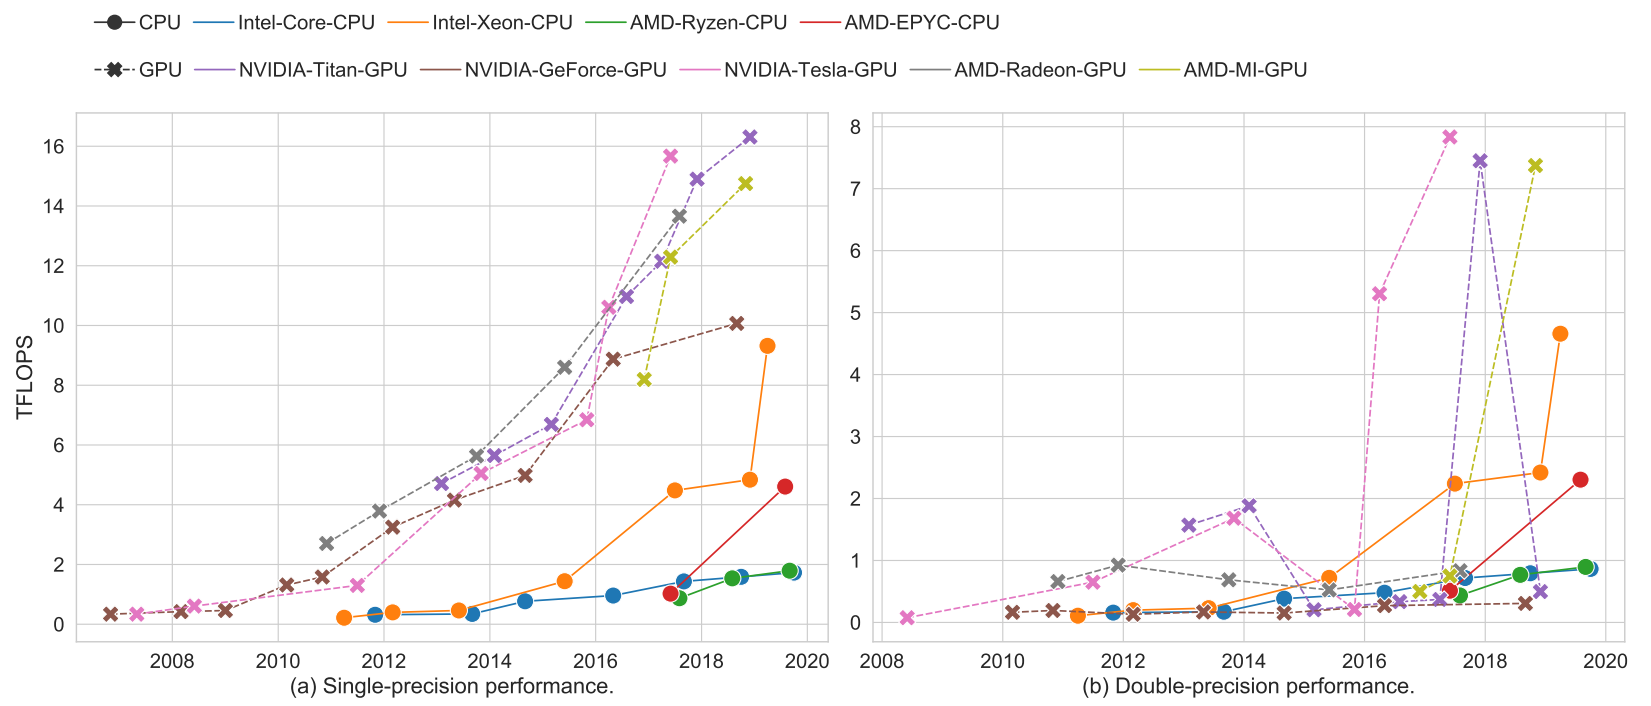
\includegraphics[width=0.9\linewidth]{gpu-vs-cpu-flops.png}
    \caption{Comparison of single-precision and double-precision performance
    between CPUs and GPUs. (Source: \cite{sun2019summarizing})}
    \label{fig:cpu-vs-gpu-flops}
\end{figure}
\todo{ask for permission to use image}

With this in mind, we can see that GPUs have been consistently faster than CPUs
for a long time (see \cite{sun2019summarizing}), which points us to the fact
that parallelization is a key factor for performance.

In short, by taking advantage of uncoupled data, parallelization can cut
execution time proportionally to the amount of computational units available,
which are often presented as ``cores''.
When talking about CPU cores, we commonly have abstractions as an attempt at
enhancing performance even further than their, more raw, physical counterparts
(see \cite{magro2002hyper} for a common abstraction technique).
We call the former, abstract cores, \textit{logical cores}, or, more commonly,
\textit{threads} and the latter \textit{physical cores}, or simply
\textit{cores}.
The same concept applies to GPUs, but often with a different nomenclature
depending on the manufacturer of the chips.
But we also ought to be careful when comparing raw component numbers between
different GPUs, as hardware design differences across manufacturers can be
more significant than in CPUs.

Although it is not always possible to convert a \textit{serial} task into a
parallelized one, some routines, such as those from linear algebra, can be
thoroughly optimized from their most basic operations, which are often
performed in uncoupled data a great many number of times -- it is, of course,
the perfect candidate for parallelization.
The GPU is one such hardware that is optimized for these tasks, and has been
gaining wide adoption in various markets -- more importantly to us, in science,
especially with the growing popularity of machine learning.
We can clearly see that it outperforms CPUs in such tasks, as shown in
\cite{buber2018performance}.

\subsubsection{Open source usage in science} \label{sec:motivation:floss-in-science}

Contemporary science's reliance on software is a relatively new phenomenon.
But such software does not seem to be held at standards as high as more
traditional content (see \cite{sufi2014software}).
It is also important to notice that it is often developed by researchers
inexperienced with real world development practices and, as such, it often
lacks the quality and robustness that one would expect for long-term
sustainability (see \cite{carver2022survey}).

One particular development strategy that appeals to modern scientific standards
is that of open source, in which the code is fully available to the public.
Most obviously, as open-source software is auditable, it becomes easier to
verify reproducibility of scientific results created with it (see
\cite{barba2022defining}), but this also allows for early collaboration between
researchers and developers, which can lead to better software design and
performance (see \cite{wilson2014best}).

Building on the practice of open source we also have \textit{free software}
(commonly denoted by FLOSS or FOSS): a development ideology that focuses around
volunteer work and donations, criticizing corporate interests, and is usually
accompanied by permissive or \textit{copyleft} licenses.
There is emerging work on the role of FLOSS in science, such as
\cite{fortunato2021case}, and some initiatives which praise a similar approach
(see \cite{katz2018community, barker2022introducing}).
It is, therefore, in our best interest to explore just how much of the current
scientific tooling is composed of free or open-source software, and to also
look for bottlenecks, where the community is not providing appropriate support
for those applications.

\subsection{Proposal} \label{sec:intro:proposal}

Distinct pieces of software usually communicate with each other through an
\textit{application programming interface} (API), which allows for the exchange
of information among them in an organized and standardized manner.
GPUs are usually coupled to the rest of the operating system (OS) with a
\textit{graphics API}, which should provide a smooth bridge from high-level
code to the actual hardware, with some APIs abstracting more than others or
providing different functionality.
Such APIs exist precisely because of them being independent pieces of hardware,
needing to be commanded as a separate entity.
Given the complexities that arise from hardware specifics, abstractions are a
must, so that we can have precise control of what matters to us without
compromising performance, leaving it up to vendors to implement such APIs on
their drivers in an optimal manner.
Thus, we can see that the choice of API is a crucial decision for the
performance of a given application, and it is important to have a good
understanding of the trade-offs that come with each one.

\subsubsection{Compilers} \label{sec:proposal:compilers}

We refer to \textit{code} as a meaningful, possibly executable, piece of text.
All code is, to a varying degree, abstracted away for the programmer, and needs
to be understood and translated to some format more useful to silicon.
These steps are performed by an interpreter or a compiler.

In the context of GPU programming we write \textit{shaders} or \textit{kernels}.
They are written in, unimaginatively, \textit{shading languages} or
\textit{kernel languages}, respectively.
Those are usually a subset of C-like languages, with some extensions to support
the specific needs of the API of interest.
Common examples include GLSL and HLSL, but those are actually a small part of
GPU utilization as, for the most part, control of its routines is still
performed on the CPU.
Graphics APIs provide such control to the programmer, as they are made to
orchestrate the entire pipeline: from managing and compiling the shaders to
synchronizing CPU and GPU and even GPU cores amongst themselves.

Of course, calls to the graphics card are not free, and shader code also has to
be compiled anyway, so during this process it undergoes further optimizations
in, roughly, two steps:
\begin{enumerate}
    \item The code is parsed and transformed into an \textit{intermediate
        representation} (IR) which can then be optimized by the compiler using
        generic directives (i.e. independently of the target hardware);
    \item The IR is, then, translated into the target machine code, and can
        also optimized, again, for the target architecture.
\end{enumerate}
The two translation steps are generally known as \textit{front-end} and
\textit{back-end} of a compiler. After those steps the shader can finally be
sent to the GPU.
In Linux this is a small part of the execution of a shader, as we can see in
Figure \cref{fig:linux-gs}, represented by Mesa -- Linux's standard userspace
graphics driver provider.

\begin{figure}[H]
    \centering
    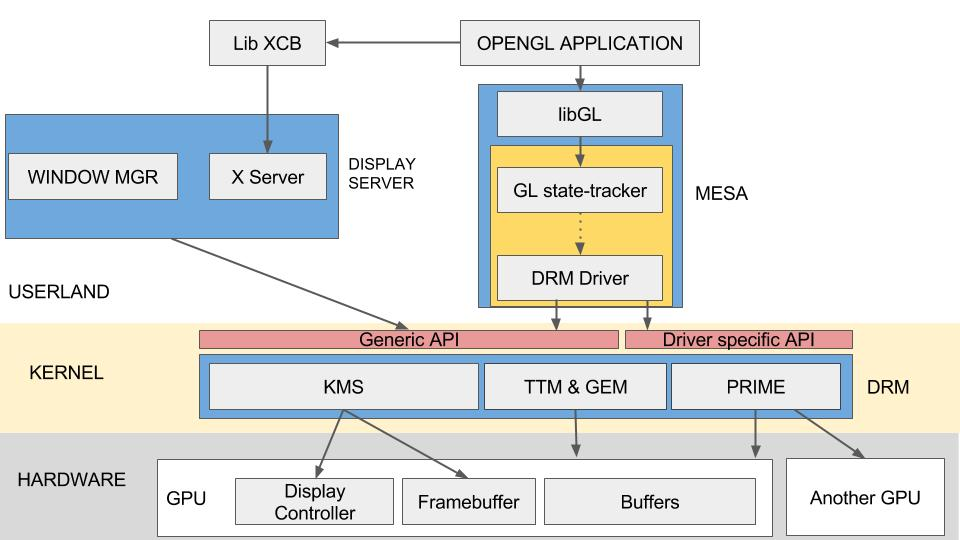
\includegraphics[width=0.8\linewidth]{linux-stack.jpeg}
    \caption{The graphics stack used in Linux kernel-based operating systems.}
    \label{fig:linux-gs}
    \end{figure}
\todo{insert image license}

\begin{figure}[H]
    \centering
    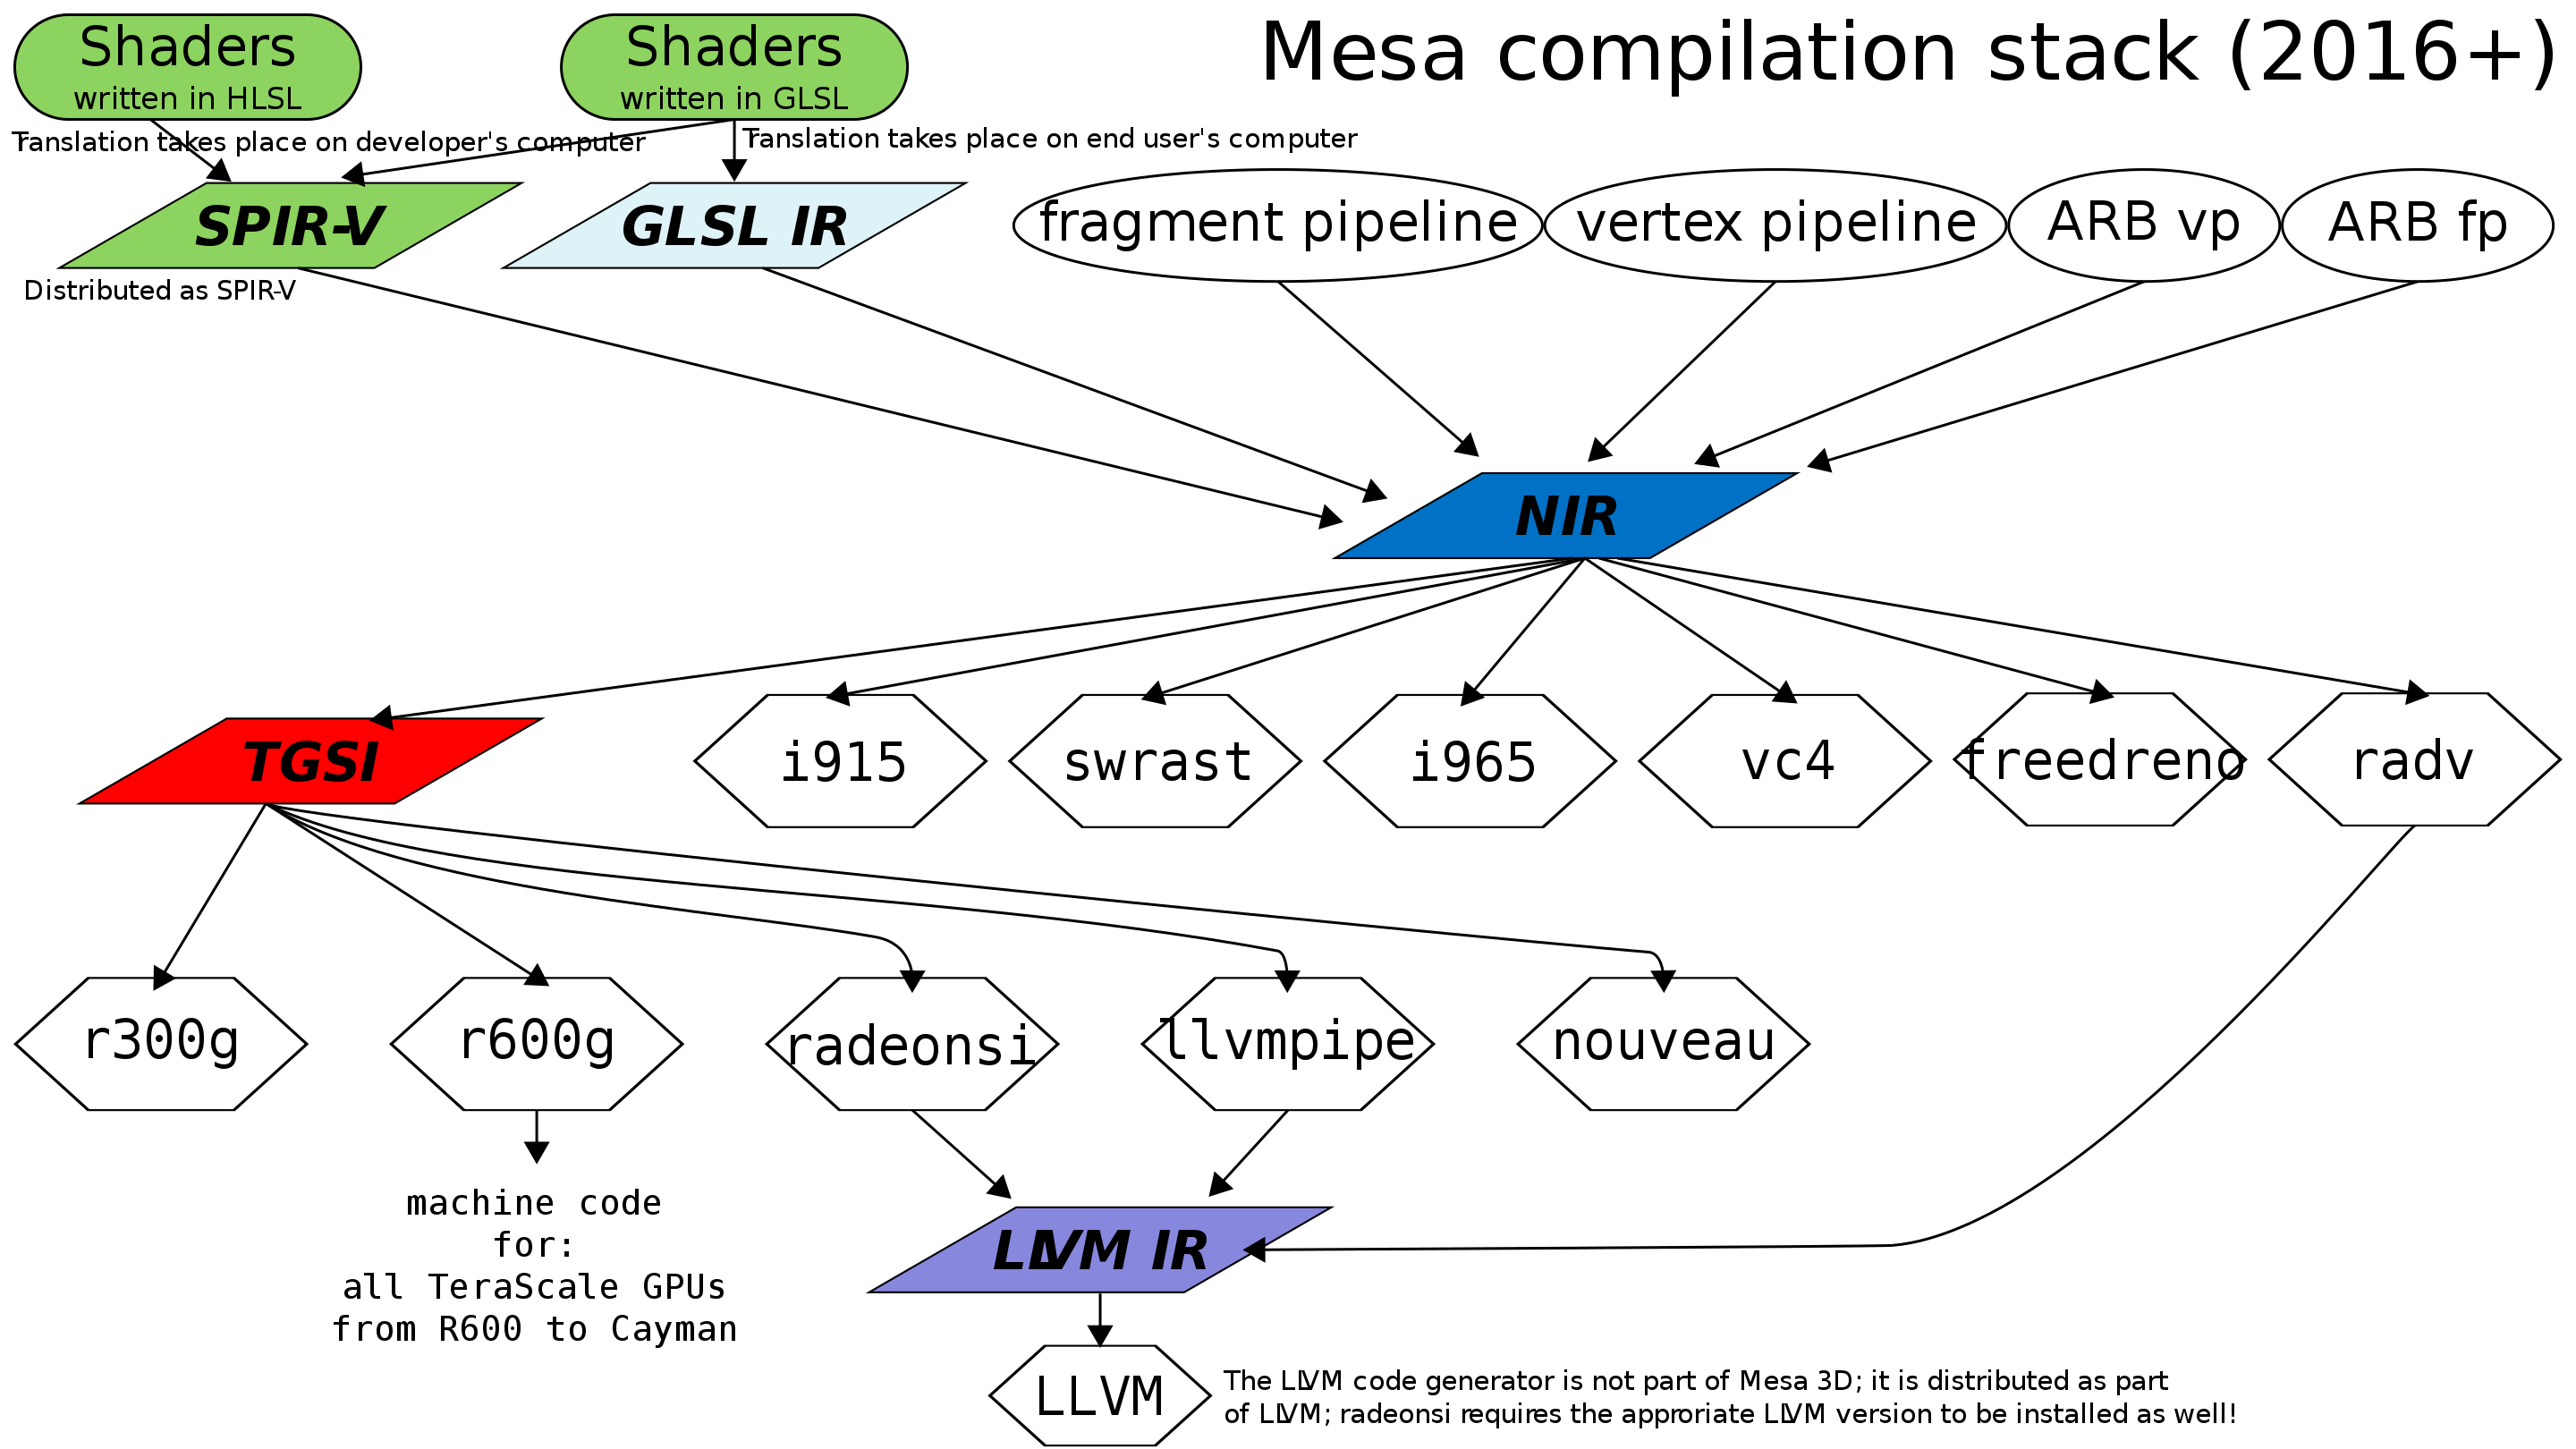
\includegraphics[width=0.8\linewidth]{mesa.png}
    \caption{Most recent compilation pipeline used by Mesa, the software
        responsible for providing open source implementations for the userspace
        part of the Linux graphics stack.}
    \label{fig:mesa-cs}
    \end{figure}
\todo{insert image license}

\subsubsection{A comparison of open source and proprietary graphics APIs} \label{sec:proposal:gapis-comparison}

\todo{Get literature on this. I found some blog posts and articles, but nothing
      that seems to be a reputable source.}

In the context of GPGPU, \textbf{CUDA} -- a proprietary API
projected and maintained by NVIDIA -- has a significantly more widespread
adoption than any other API, proprietary or not.
On the one hand, most open source alternatives that provide the same
functionality are either in their infancy or have not provided what was needed
to replace CUDA, examples are, respectively, HIP by AMD, and OpenCL by the
Khronos Group.
On the other hand, we have Vulkan as an alternative.
It has a great upside of being more general, as it is not proposed solely for
computation but also as a standard graphics API, providing display
functionality.
Thus, manufacturers (including NVIDIA) have implemented this standard and
optimize it proactively, which is exactly what OpenCL has lacked since its
release.

% Given the perception of NVIDIA's technologies being the go-to choice for
% scientific applications.

\todo{Drop back-of-the-envelope calculations and analyze data from GitHub API}
We can estimate CUDA's ``literature-share'' with back-of-the-envelope
calculations, as this fact lacks research to back it:

\begin{enumerate}
    \item We query \href{https://github.com}{GitHub} for
        \verb|cuda language:cuda language:c language:c++ stars:>=5 followers:>=5|
        so that we can see how many projects have been specifically designed to
        leverage the CUDA API, and get 1835 results.
    \item Now we make a similar query for the other, open source, APIs, and get
        680 results for OpenCL and 895 for Vulkan. Results for HIP are not as
        reliable as ``HIP'' is often part of another word, and it only gives is
        about 100 results, so there is not enough room to isolate the noise.
    \item As Vulkan is, for the most part, not used for GPGPU, we can rule out
        at least 2/3 of results, which gives us $ 1835 / (680 + 895 * 1/3 +
        1835) \gtrsim \qty{65}{\percent} $ of potentially relevant applications
        supporting CUDA.
\end{enumerate}

It is clear, then, that there is a great disparity amongst API adoption rates,
especially taking into account the popularity of the applications in each
group.

Given that Vulkan tries to cover more ground than any other API, it also has a
significantly steeper learning curve as compared to CUDA, making its adoption
more challenging when compared to other alternatives.
OpenCL-related tooling has recently gained more focus amongst open-source
software consultancies, as we can see in \cite{MachineL70:online}.

\subsection{Objectives} \label{sec:intro:objectives}

Given approximate usage statistics of CUDA, we lay down some of our objectives:

\begin{enumerate}
    \item\label{obj1} Get a more precise figure of the usage of
        graphics-accelerated open-source software used in scientific
        applications.
    \item\label{obj2} Find out how CUDA stands out from its open source
        alternatives.
    \item\label{obj3} Find ways to overcome such differences and make it easier
        for maintainers' to add support for open source APIs.
\end{enumerate}

We choose to analyze \textbf{Vulkan} and \textbf{OpenCL} as they are the most
prominent open source alternatives to CUDA, and we will also take a look at
\textbf{HIP} as it is the most recent addition to the list.
Both Vulkan and OpenCL are Khronos Group standards, of which more than 170
companies are members, including AMD, ARM, Intel, NVIDIA, and Qualcomm.
Their API specifications are open and have ample documentation and adoption,
which makes them a good choice for our analysis.
HIP (Heterogeneous-Compute Interface for Portability) provides a solution to
ease the transition from CUDA to more portable code, thus making it interesting
to us as well.

\section{Methodology} \label{sec:methodology}

In October 2022 I have attended
\href{https://indico.freedesktop.org/event/2/page/11-overview}{X.Org Developers Conference 2022}
in order to present another project I have developed in
\href{https://summerofcode.withgoogle.com/programs/2022/projects/6AoBcunH}{Google Summer of Code 2022}.
While it was unrelated to the topic of this thesis, I got to meet many people
from the open-source graphics community, and learn much about the state of the
art when it comes to open source graphics APIs, namely with respect to their
usage and development.

In the MAC0414 course, I have learned many things about the theory behind
compilers, mainly through \cite{sipser1996introduction}, which should help me
understand the compilation process of GPU code, and how the pipeline is
structured for each API.
Then, in the MAC0344 course I have learned about the main aspects guiding
performance in modern hardware, and also about some of their most common
optimizations.
I have also started to learn about graphics programming in general, starting by
OpenGL, which is the most common API, and should provide a good basis for
understanding both Vulkan and OpenCL.
I have also started to look up literature on benchmarks and performance
analysis.

\subsection{Statistics} \label{sec:methodology:statistics}

So far, we have made some progress on \cref{obj1} by analyzing popular
graphics-accelerated projects using topic modeling.

\subsubsection{Data collection} \label{sec:methodology:statistics-data}

First we assumed that most scientific applications use CUDA, and then by
looking up all projects with the \verb|Academia/Higher Education|,
\verb|HPC/Supercomputing|, and \verb|Healthcare/Life Sciences| labels on
\href{https://nvidia.com/en-us/gpu-accelerated-applications}{NVIDIA's list of accelerated apps}
we got a list of 494 projects that should be using CUDA and, as recognized by
NVIDIA, are at least somewhat relevant.
From the 494 projects available with the tags above, we have narrowed the list
down to 141 projects that are open source and use \verb|git| as their version
control system through manual inspection.
After that, following \cite{zheng2018measuring}'s methodology, we gathered the
repositories' \verb|README| files and removed sections that were not relevant to
the project, such as \verb|Installation|, and \verb|License|, then we used
Latent Dirichlet Allocation (LDA) to group projects into topics, which should
help us find out what each project is about.

\subsubsection{Data analysis} \label{sec:methodology:statistics-analysis}

As a first step, it was necessary to clean the data further, as there are many
unnecessary words that would skew the results (such as \verb|the|, \verb|and|,
etc.) which are generally known as \textbf{stop words}.
We also remove symbols, such as punctuation, numbers and very short words, as
they are not relevant to the analysis.
Then it is necessary to tokenize the data, that is, to break the text into
smaller pieces, called tokens.
Then we lemmatize it, a process by which we reduce each word to its root form,
so that, for example, \verb|computing| and \verb|computations| are both reduced
to \verb|compute|.
This makes analysis easier, as it reduces the number of words to a more
manageable amount, and also makes it easier to compare words that are similar
in meaning.

We then store the results of preprocessing in a count vector, which is a matrix
where each row represents a document, and each column represents a word, and
the value in each cell is the number of times that word appears in that
document.
That way we can abstract away from the order of the words, thus making it
easier to compare documents.
In this step we also remove words that appear in less than $\qty{10}{\percent}$
of documents, or in more than $\qty{90}{\percent}$ of them, as they are either
too common or too rare to be relevant to the analysis.

After that, we use \textit{latent Dirichlet allocation} LDA to group the
documents into topics, which is a probabilistic model that assumes that each
document is a mixture of topics, and each topic is a mixture of words.
LDA assigns every word in every document to a topic randomly at first, then
updates its assignments according to the probability of a word belonging to a
topic and the probability of a topic being assigned to a word.
It will then repeat this process until it converges, so that the topics do not
change anymore.
We train the model assuming a number $N$ of topics.

Of course that are other hyperparameters that can be tuned, such as the
densities for how many words should be in each topic ($\eta$), and for how many
topics should be in each document ($\alpha$).

\subsubsection{Hyperparameter tuning} \label{sec:methodology:statistics-hyper}

We analyze \verb|gensim|'s hyperparameters by looking taking a range of them
and training the model as usual, then we look at the \textit{coherence score},
which is a metric that measures how well the model is able to group words that
are semantically linked.

First, let's look at the coherence score for different numbers of topics, see
\cref{fig:coherenceXtopics}.
We can see that the coherence score is highest for $N = 8$, so we will use that
value for the rest of the analysis.

\begin{figure}[H]
    \centering
    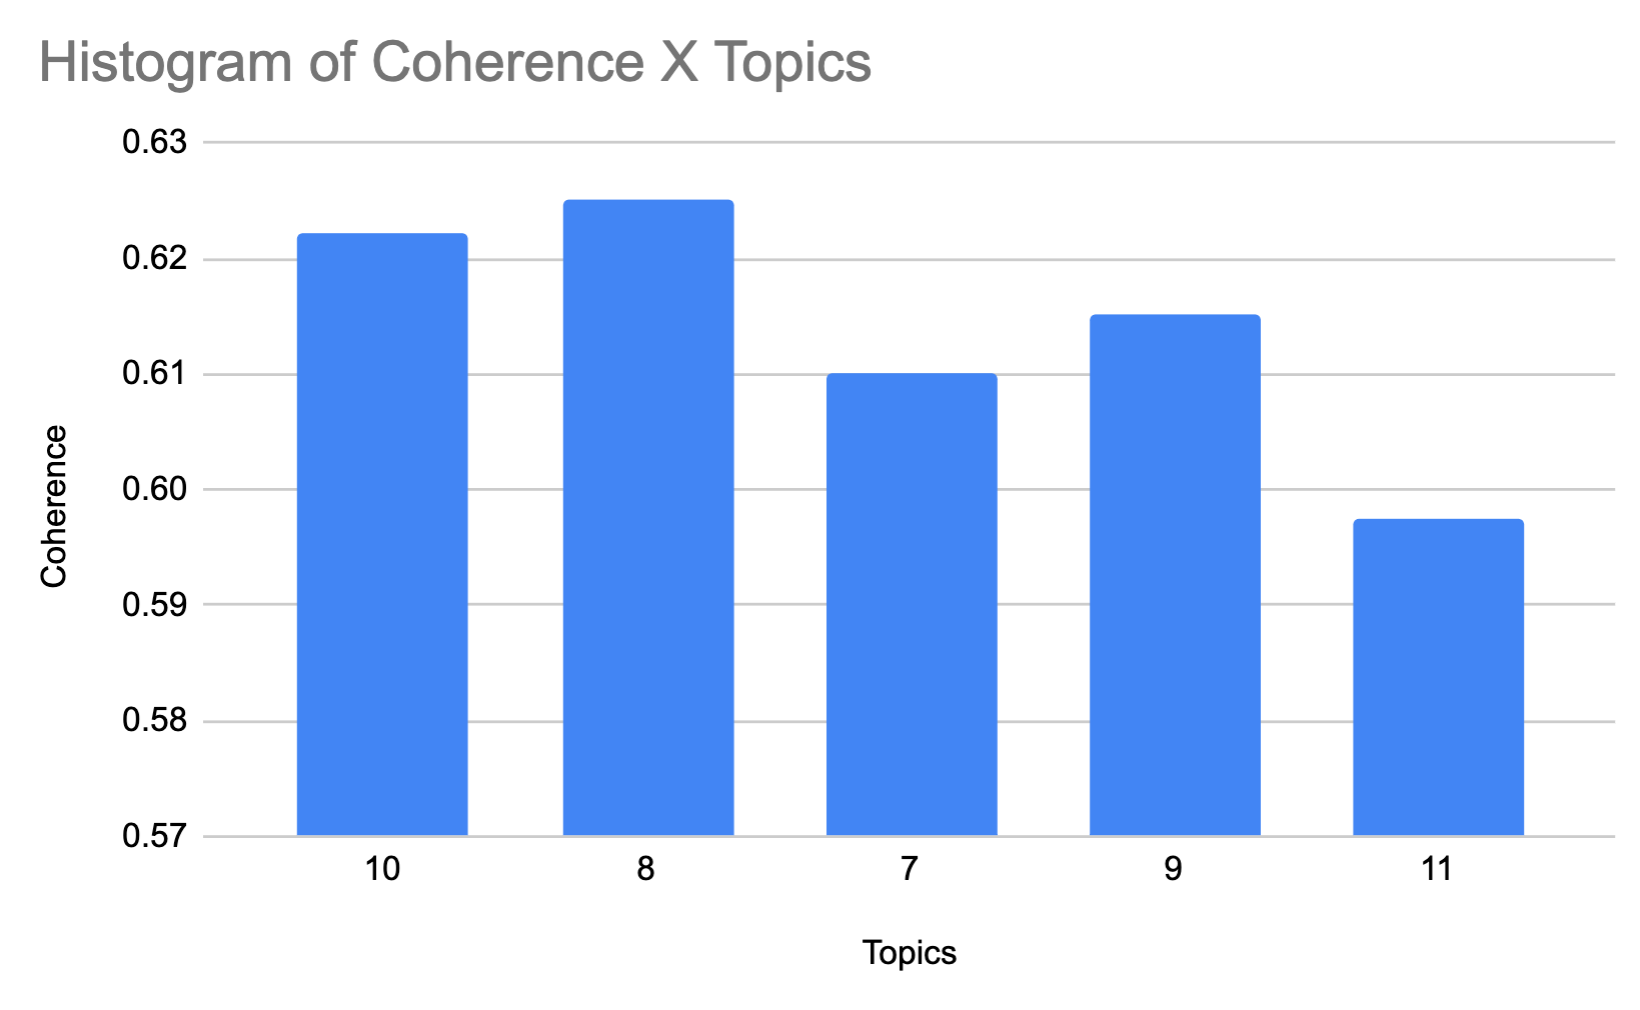
\includegraphics[width=0.7\linewidth]{coherenceXtopics.png}
    \caption{Average coherence score for a range of topics.}
    \label{fig:coherenceXtopics}
\end{figure}
\todo{update graph}

Now, for the other parameters, it's interesting to look at different samples of
the data so we don't overfit the model to the data.
Overfitting is a problem that happens when the model is too complex for the
data, and it memorizes the data instead of learning the underlying patterns.
So by optimizing results for the whole corpus but also for a smaller sample, we
can avoid overfitting.
In figures \cref{fig:75p-coherenceXalpha-eta} and
\cref{fig:100p-coherenceXalpha-eta} we can see that the coherence score is
highest for $0.4 \leqslant \alpha \leqslant 0.7$ and
$0.1 \leqslant \eta \leqslant 0.4$.
As the step between these values is $0.3$, we can't really tell which value is
optimal, so we reduce the range of both parameters to the intervals we found to
be most promising, and look at the coherence score using a smaller step.
Notice it's often a good idea to make ranges a little bigger, so that we can
take into account optimal values that might be near the edges of the range.

\begin{figure}[H]
    \centering
    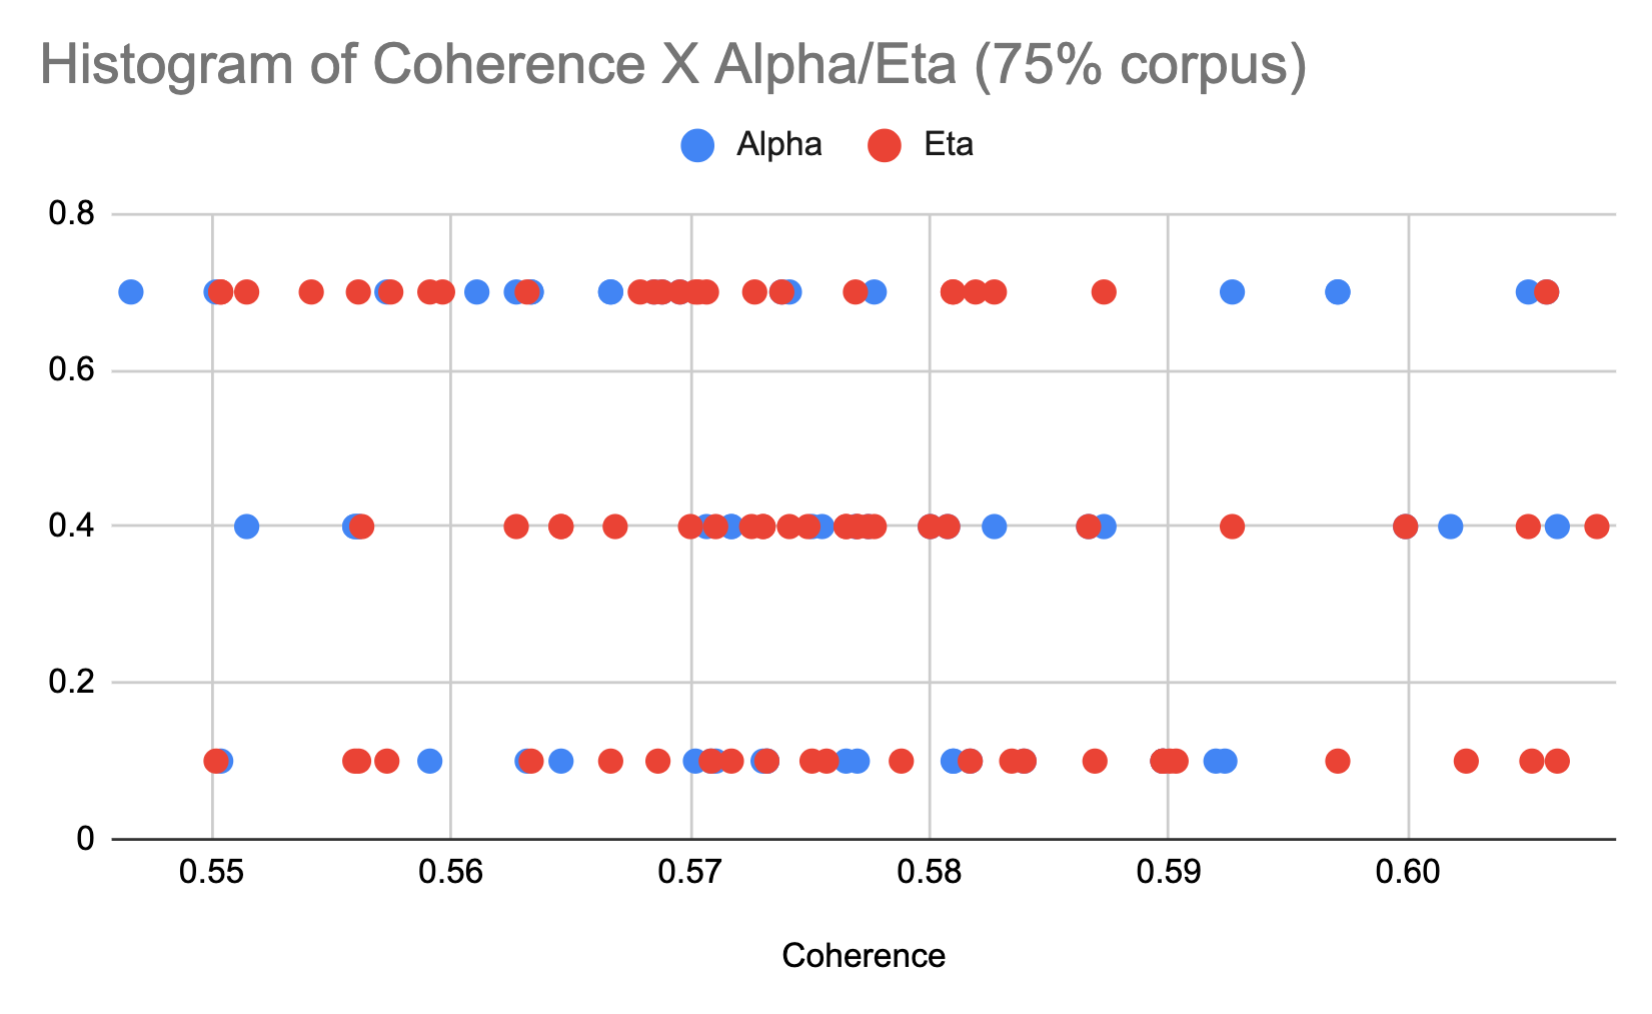
\includegraphics[width=0.7\linewidth]{75p-coherenceXalpha-eta.png}
    \caption{Average coherence score for different $\alpha$ and $\eta$ using
        \qty{75}{\percent} of the data (corpus).}
    \label{fig:75p-coherenceXalpha-eta}
\end{figure}
\todo{update graph}

\begin{figure}[H]
    \centering
    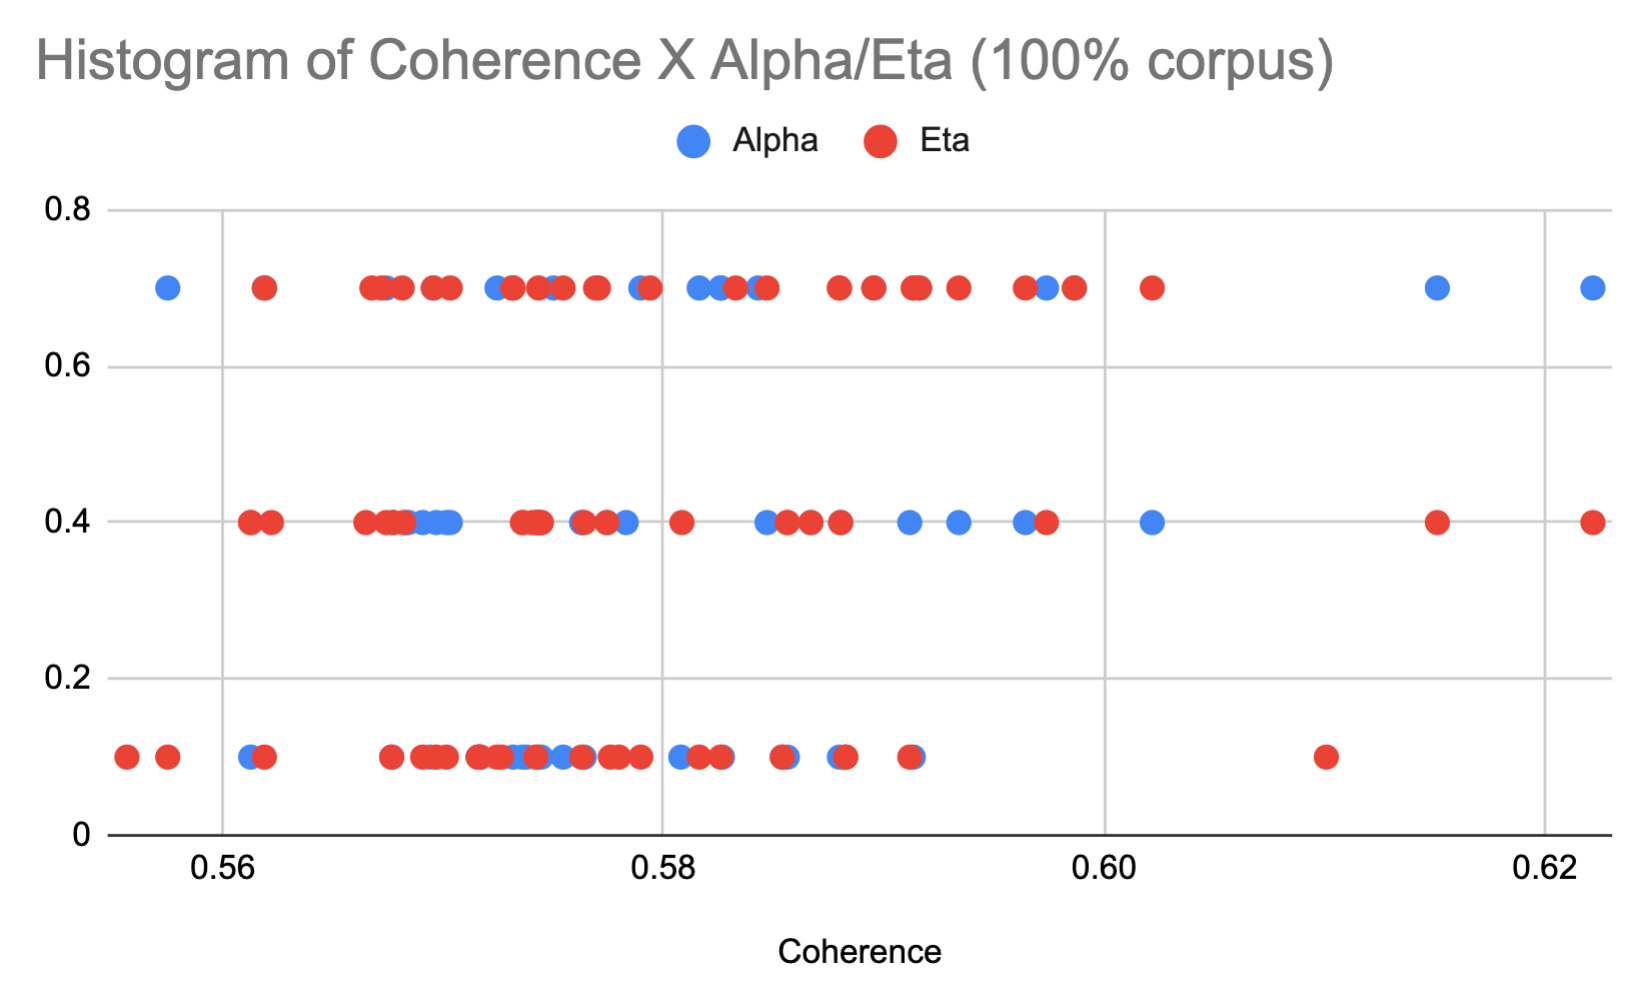
\includegraphics[width=0.7\linewidth]{100p-coherenceXalpha-eta.png}
    \caption{Average coherence score for different $\alpha$ and $\eta$ using
        all of the data (corpus).}
    \label{fig:100p-coherenceXalpha-eta}
\end{figure}
\todo{update graph}

We continue narrowing down the intervals for $\alpha$ and $\eta$ up to a
precision of $0.01$, for which the coherence score seems stable for neighboring
values.

\subsubsection{Implementation issues} \label{sec:methodology:statistics-issues}

We started by using the \verb|gensim| library's implementation of LDA, namely
the \verb|LdaMulticore| class to train the model, and use the
\verb|CoherenceModel| class to calculate the coherence score and find the best
hyperparameters.
\verb|LdaMulticore| is a parallel implementation of LDA, and in \verb|gensim|
it takes in a \textit{Bag-of-Words} (BoW) and a \textit{corpus}.
The BoW is a list of lists, where each list is a document, and each document is
a list of tuples, where each tuple is a word and its frequency.
The corpus is a list of the indexed words existent in the documents, in which
repetitions have been removed.
We then used the \verb|pyLDAvis| library, which is a visualization tool for LDA
models, but it did not work too well, as the topics were either too broad or
too overlapping, so we decided to try using the \verb|scikit-learn| library
instead, which uses a different algorithm to train the model.
Then, using the same visualization library we were able to get better results,
which was indicative that there was something wrong with the way we were
processing the data in some step on the attempt to use \verb|gensim|.

\begin{figure}[H]
    \centering
    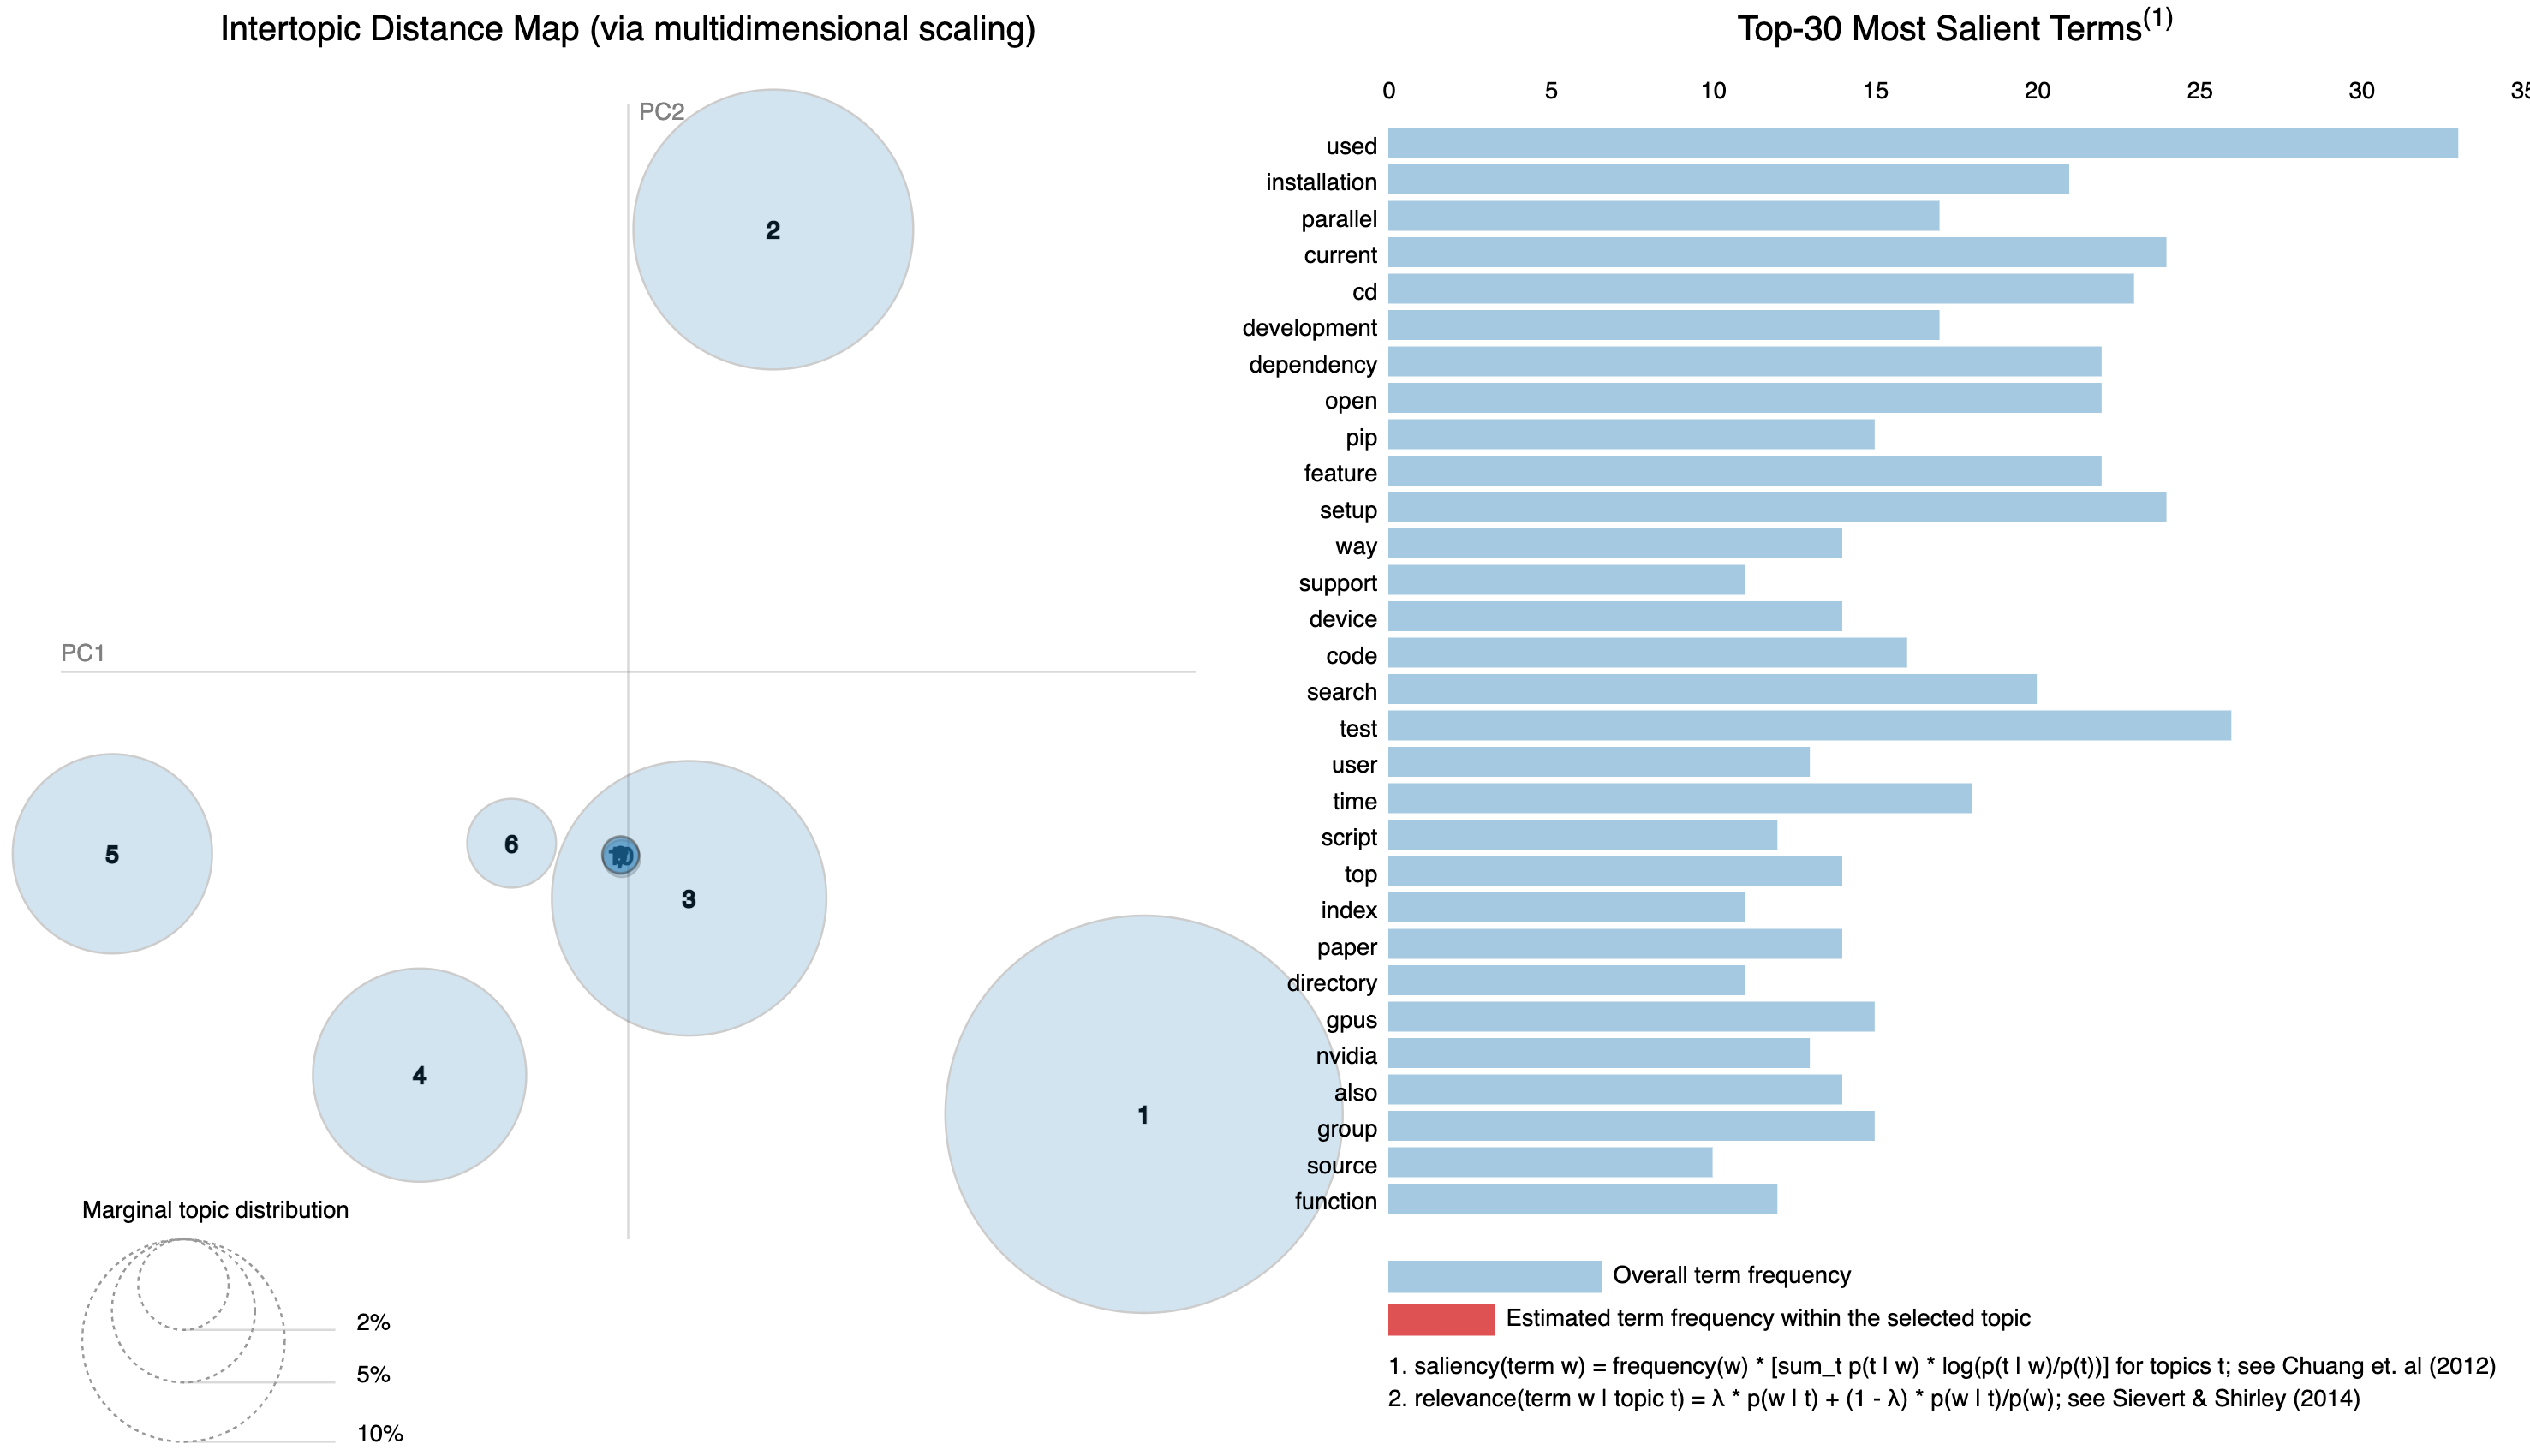
\includegraphics[width=\linewidth]{gensim-untrained.png}
    \caption{Visualization of gensim's LDA results (untrained model with
        default dimensionality reduction method).}
    \label{fig:lda_gensim_untrained}
\end{figure}
\todo{update graph}

\verb|scikit-learn|'s LDA implementation takes in a different format of the
data than \verb|gensim|, as it uses a count vector.
This required significant changes to the preprocessing steps, as we had to
incorporate the count vector into the pipeline, and also change the way we
tokenized the data (the preprocessing steps described above represent the
latest implementation).
As both models were trained with the same data, which was just converted from
the count vector to a BoW and a corpus, we were unable to find the cause of the
such a great difference in results at the LDA step.

\begin{figure}[H]
    \centering
    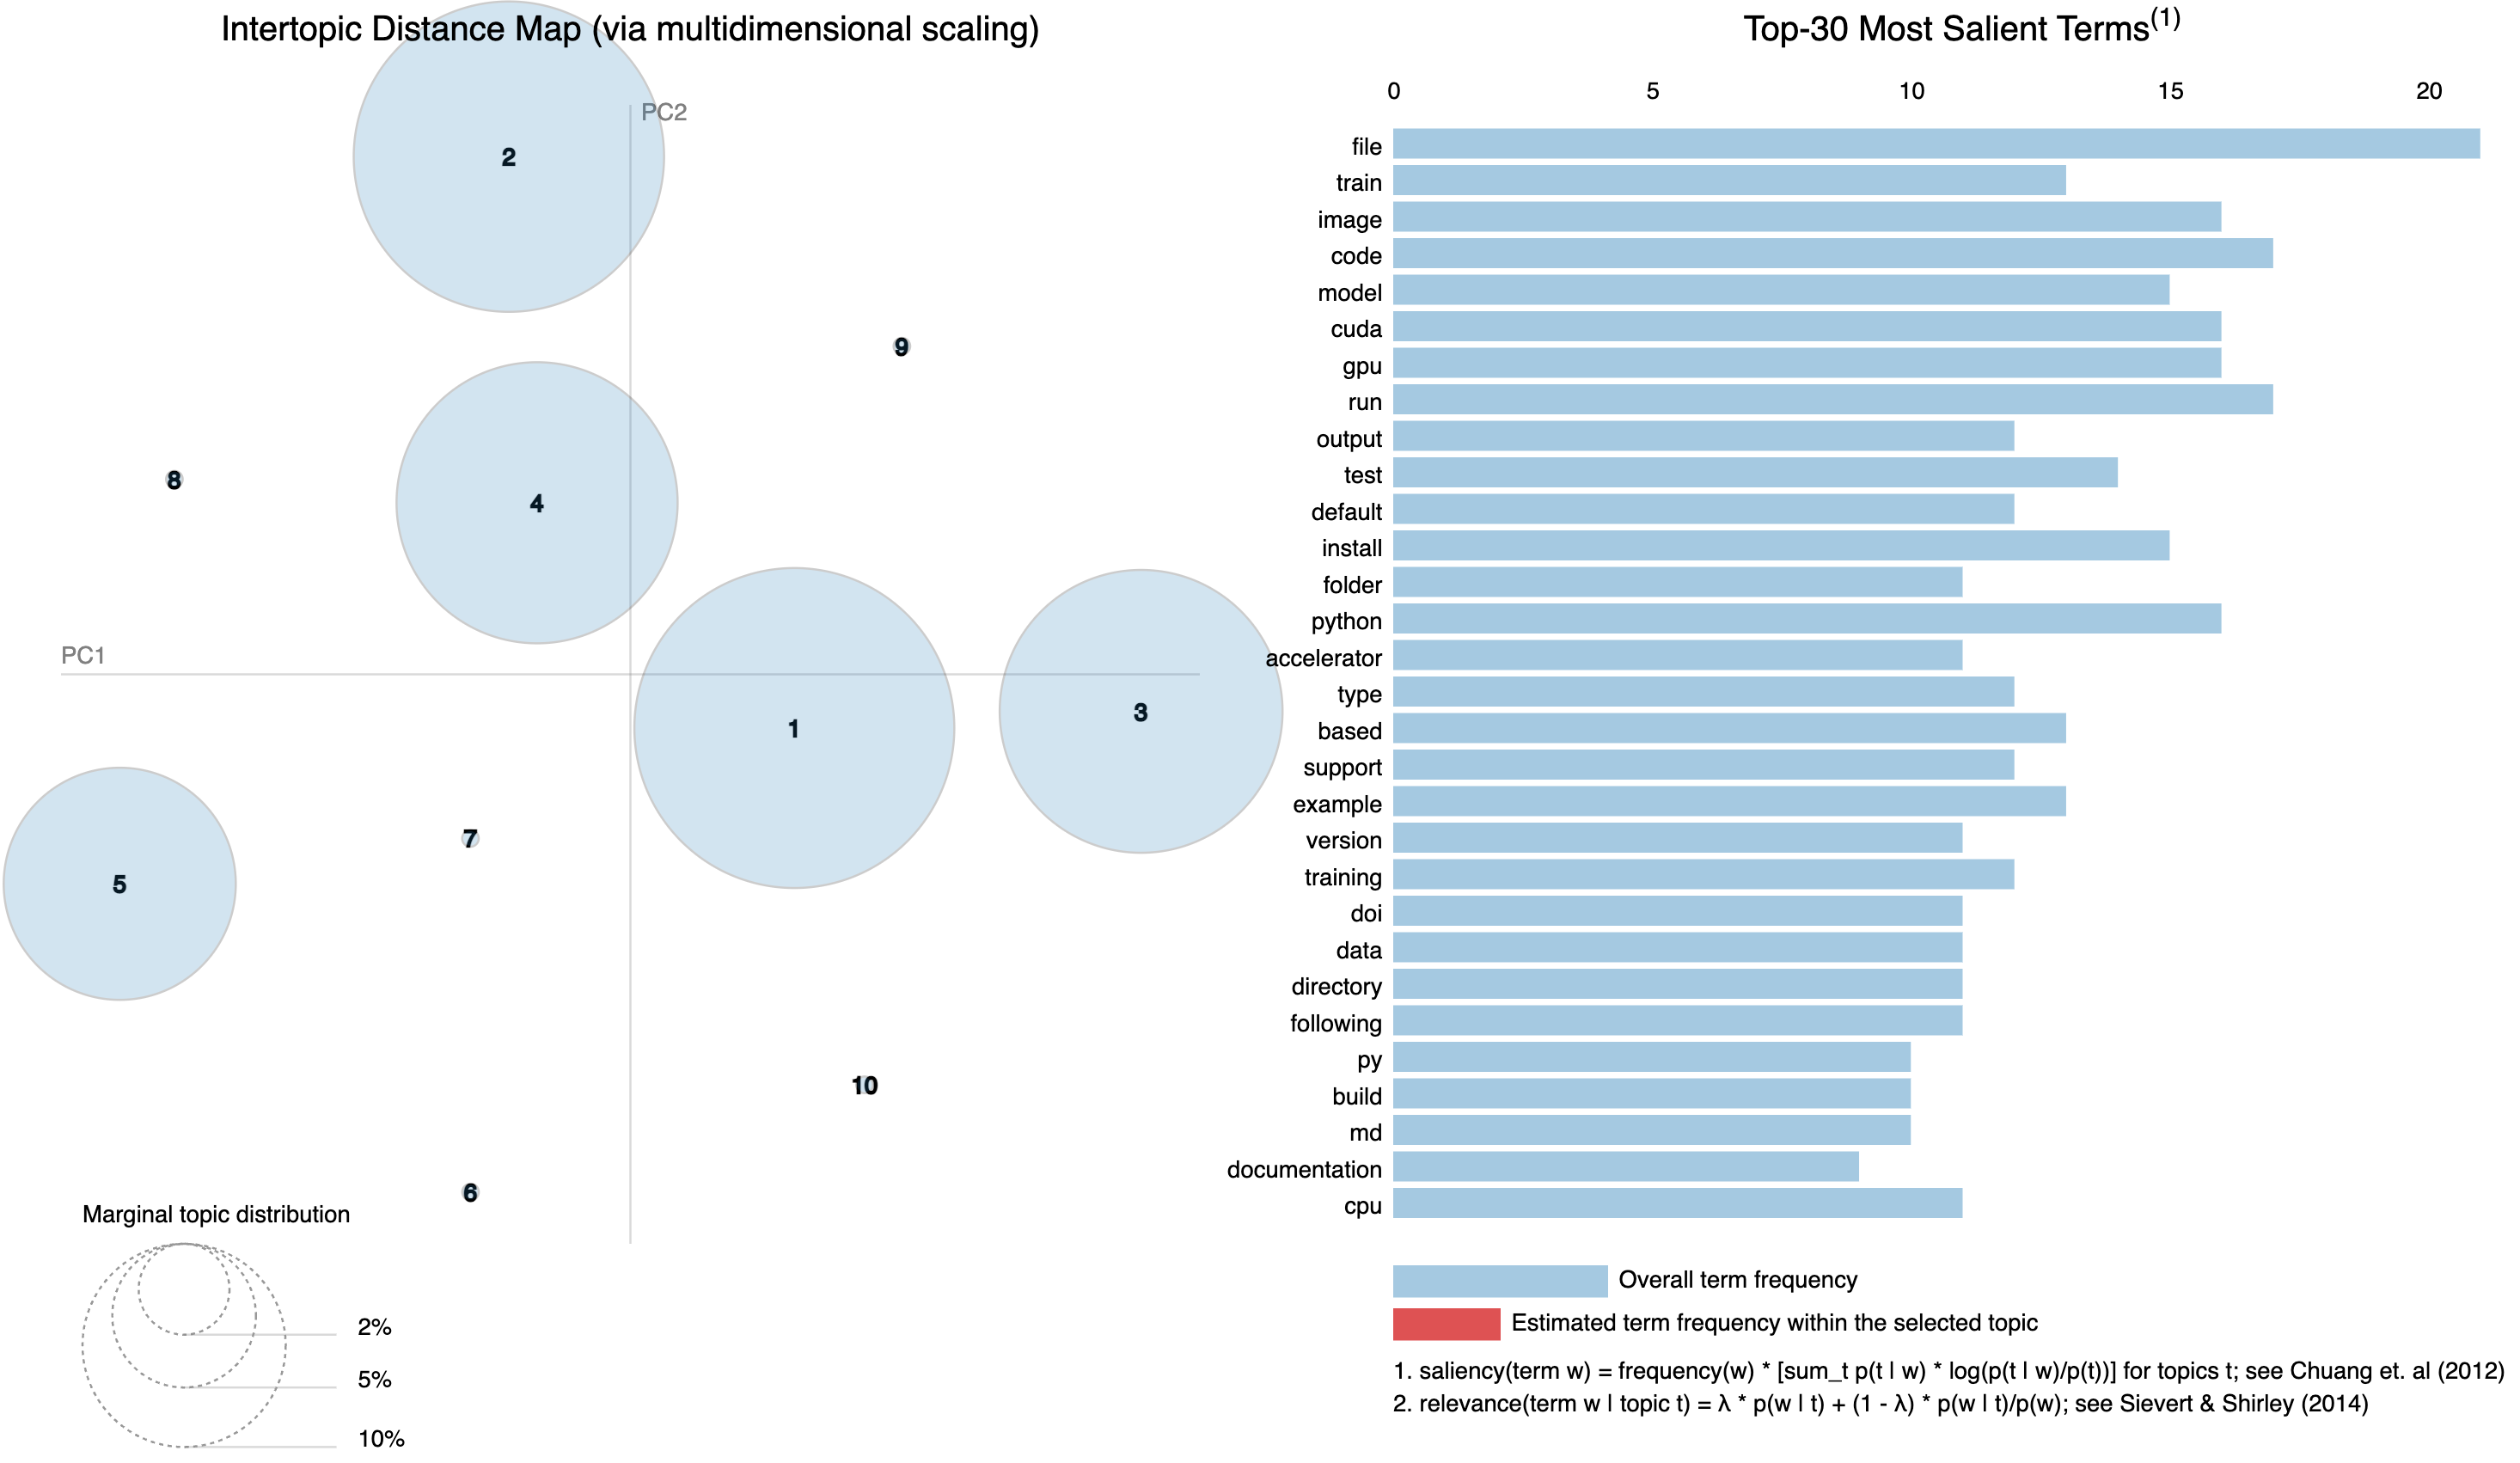
\includegraphics[width=0.95\linewidth]{sklearn-default.png}
    \caption{Visualization of SciKit-learn's LDA results (untrained model with
        t-SNE dimensionality reduction method).}
    \label{fig:lda_sklearn_untrained_mds}
\end{figure}
\todo{update graph}

\begin{figure}[H]
    \centering
    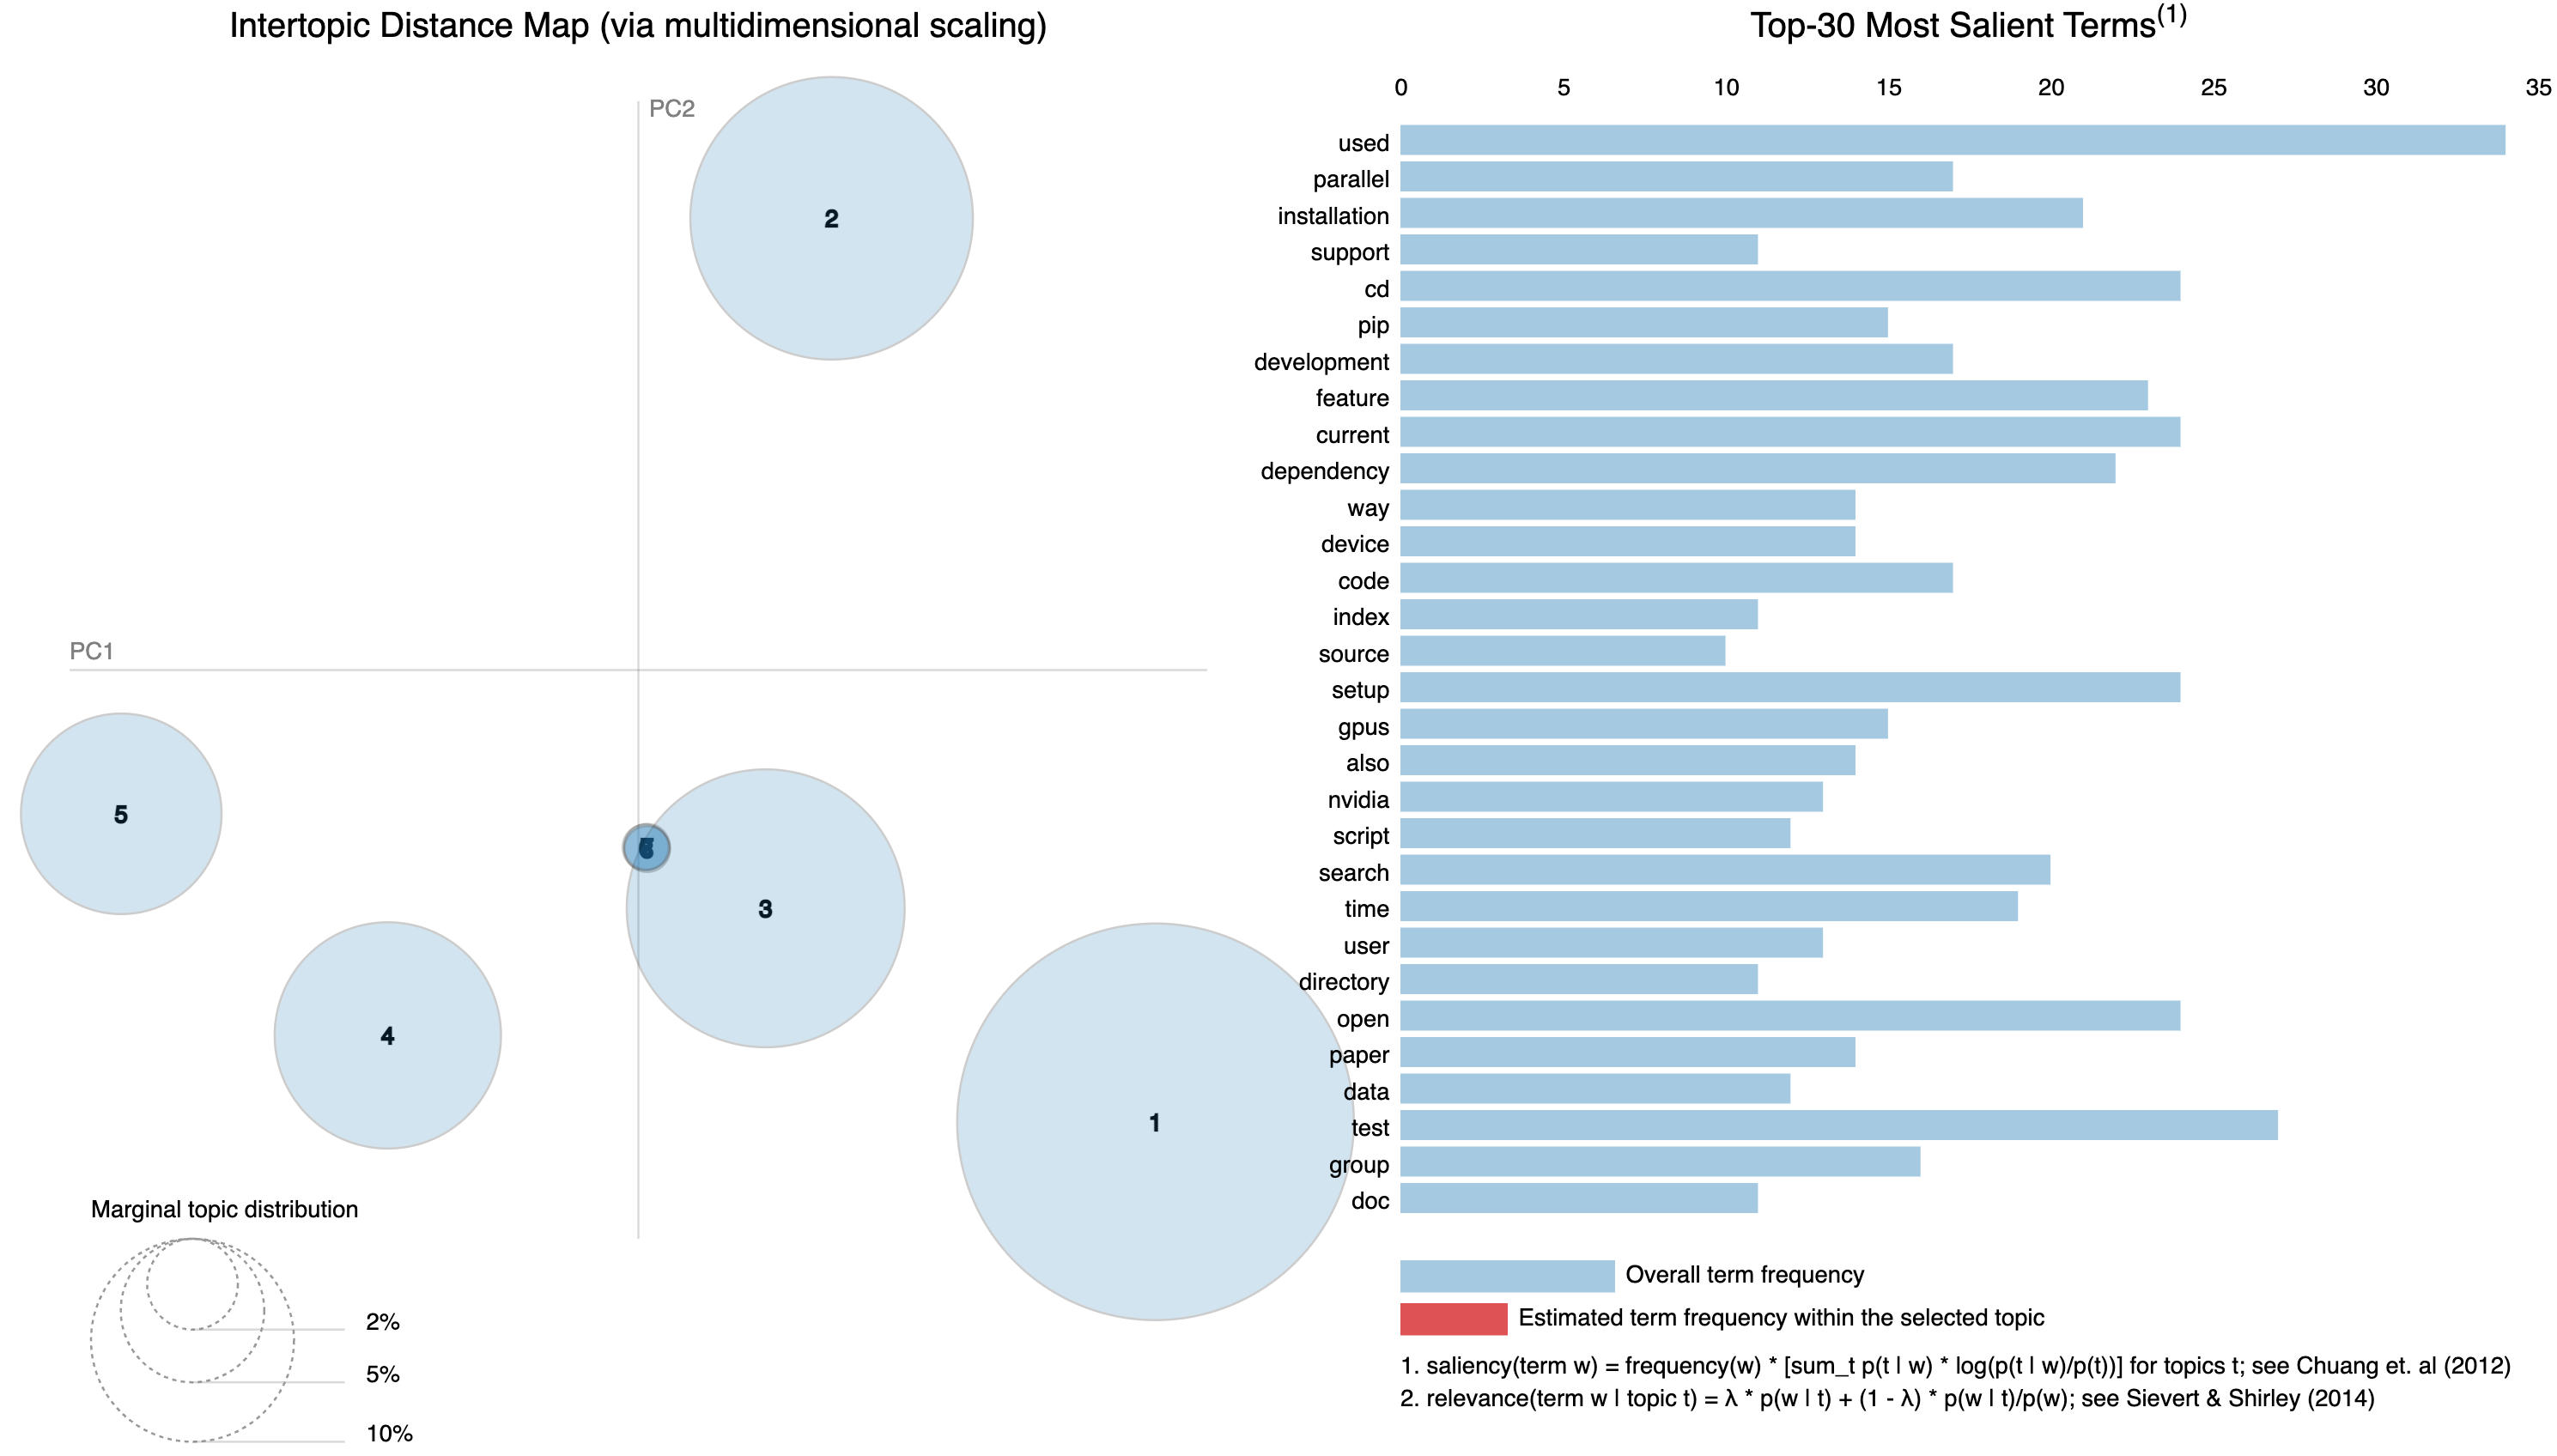
\includegraphics[width=0.95\linewidth]{gensim.png}
    \caption{Visualization of gensim's LDA results (trained model with default
        dimensionality reduction method).}
    \label{fig:lda_gensim}
\end{figure}
\todo{update graph}

We can notice that \verb|pyLDAvis| was able to generate better results with
\verb|scikit-learn|, even after tuning \verb|gensim|'s hyperparameters, as the
topics are more distinct (i.e. non-overlapping) and the words are more relevant
to the topic, as we can see in figures \cref{fig:lda_sklearn_untrained_mds} and
\cref{fig:lda_gensim}.
Upon further inspection it became clear that we were using a rather simplistic
visualization technique for \verb|gensim|'s results.
\verb|pyLDAvis|, under the hood, uses dimensionality reduction techniques,
which are needed to make the visualization work and, by default, it uses
\textit{principal component analysis} (PCoA), which does not need much manual
tweaking, but it also does not work well with sparse data, which is our case.
We were able to generate better results than either previous iteration by using
the \textit{t-distributed stochastic neighbor embedding} (t-SNE) method for
\verb|pyLDAvis| with a tuned \verb|gensim| model, as we can see in
\cref{fig:lda_gensim_tsne}.
T-SNE works well with sparse data, as it is better able to preserve local
structure, but it needs manual tuning.

\begin{figure}[H]
    \centering
    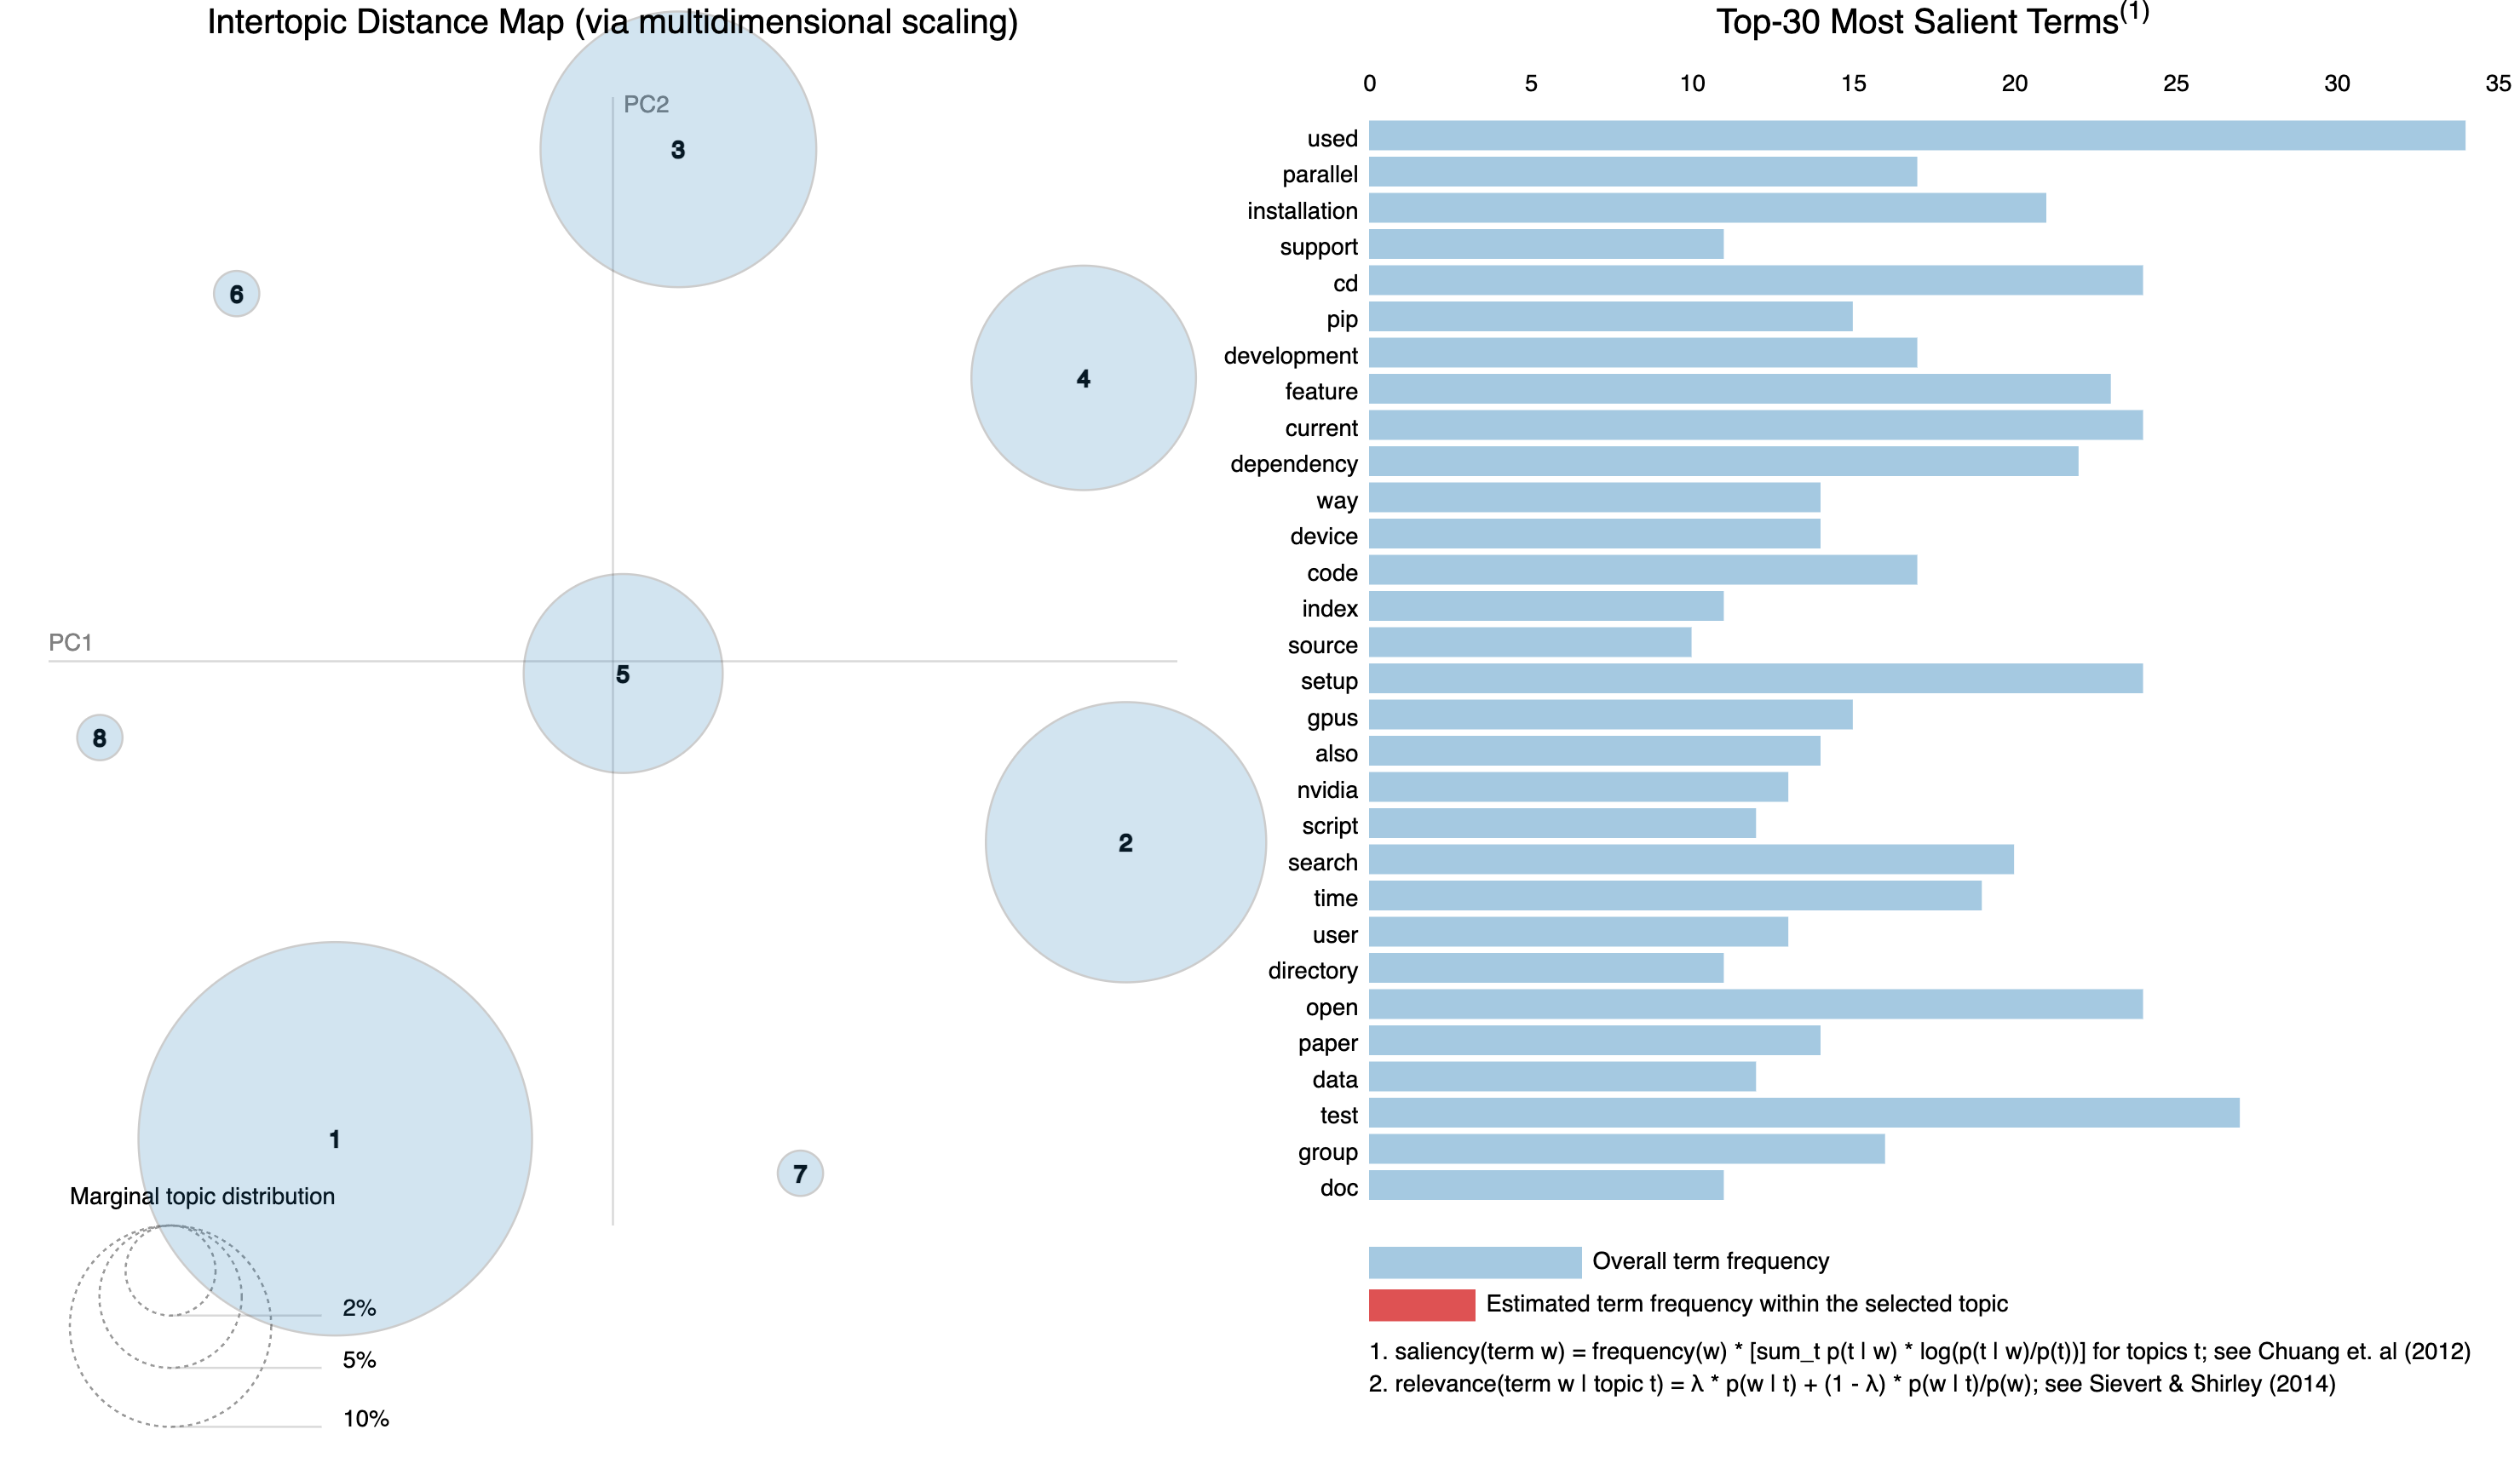
\includegraphics[width=\linewidth]{gensim-tsne.png}
    \caption{Visualization of gensim's LDA results (trained model with t-SNE
        dimensionality reduction method).}
    \label{fig:lda_gensim_tsne}
\end{figure}
\todo{update graph}

Unfortunately our results with LDA alone were not satisfying.
See \cref{sec:next-steps-statistics} for more details.

\section{Discussion} \label{sec:discussion}

By taking the most likely topic for each document, we were able to plot
\cref{fig:topic-probabilities}.
Looking at the words composing each topic, there was not a clear distinction
between them, thus we were not able to make any conclusions about the
repositories' actual subjects.
Given that \cite{zheng2018measuring}'s approach wanted to generate a
recommendation model as its main goal, we believe our analysis needs to take on
a different approach, as discussed in \cref{sec:next-steps:statistics}.

\begin{figure}[H]
    \centering
    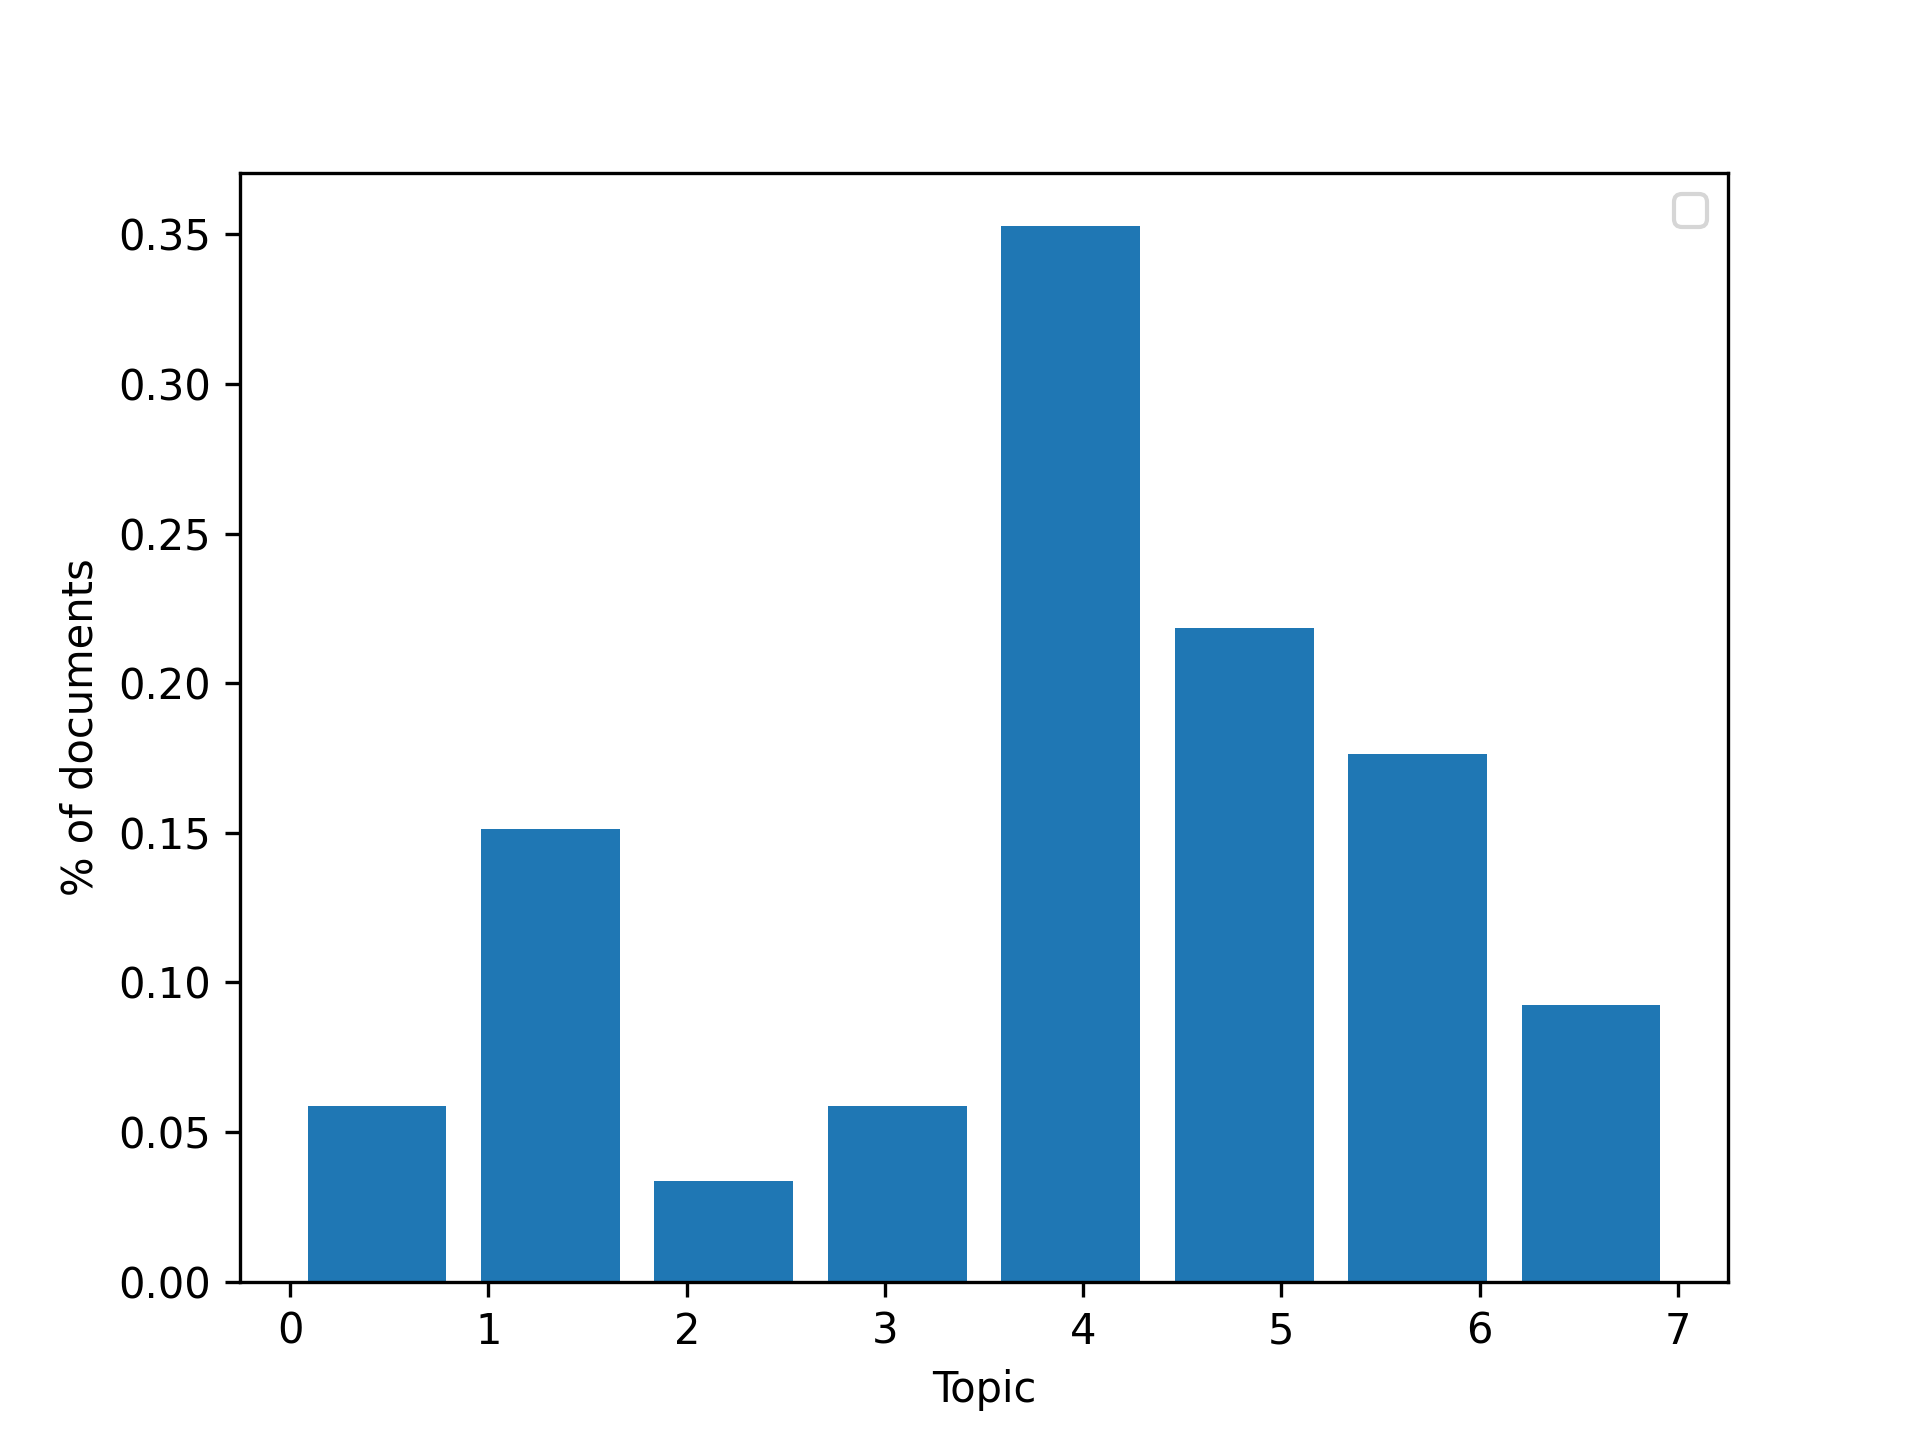
\includegraphics[width=0.7\linewidth]{topic-probabilities.png}
    \caption{Topic probability distribution the documents in the corpus.}
    \label{fig:topic-probabilities}
\end{figure}
\todo{update graph}

\section{Next steps} \label{sec:next-steps}

\subsection{Statistical analysis} \label{sec:next-steps:statistics}

\todo{i don't know what to do :)}

\subsection{Graphics APIs} \label{sec:next-steps-apis}

As we finish the statistical analysis phase, we then proceed to benchmark the
projects we have selected, giving special attention to those that implement
another graphics API besides CUDA.
We will then compare the performance between top projects in each category, and
analyze different implementations of similar routines.
This requires understanding the different APIs, and how they work.
It will also require finding useful benchmarks and tools, as well as possibly
implementing our own.

Aside from personal studies, I'll also be taking courses in parallel
programming and operating systems.
The first will be useful for learning an overview of the CUDA API as well as
for benchmarking the projects we have selected.
The second should provide the tools for interpreting the internals of the
environment which executes our compute pipelines, thus providing for a better
grasp of the orchestrations that happen at every level of execution.

\bibliographystyle{IEEEtran}
\bibliography{../../IEEEabrv,references}

\end{document}
